%$Header: /cvsroot/esrg/sfesrg/esrgpubs/acm0010/paper/acm_paper.tex,v 1.5 2003/04/08 03:57:12 dtashley Exp $

\documentclass{esub2acm}

\usepackage{amsfonts}
\usepackage{amsmath}

\usepackage{graphicx}

%%%%%%%%%%%%%%%%%%%%%%%%%%%%%%%%%%%%%%%%%%%%%%%%%%%%%%%%%%%%%%%%%%%%%%%%%%%%%%%%%%%%%%%%%%%%%%%%%%%%%%%%
%%%%%%%%%%%%%%%%%%%%%%%%%%%%%%%%%%%%%%%%%%%%%%%%%%%%%%%%%%%%%%%%%%%%%%%%%%%%%%%%%%%%%%%%%%%%%%%%%%%%%%%%
% NEW NUMBERED ENVIRONMENTS (THEOREMS, EXAMPLES, ETC.)                                                 %
%%%%%%%%%%%%%%%%%%%%%%%%%%%%%%%%%%%%%%%%%%%%%%%%%%%%%%%%%%%%%%%%%%%%%%%%%%%%%%%%%%%%%%%%%%%%%%%%%%%%%%%%
%%%%%%%%%%%%%%%%%%%%%%%%%%%%%%%%%%%%%%%%%%%%%%%%%%%%%%%%%%%%%%%%%%%%%%%%%%%%%%%%%%%%%%%%%%%%%%%%%%%%%%%%
\newtheorem{algorithm}{Algorithm}

\newtheorem{example}{Example}

\newtheorem{mytheorem}{Theorem}

%%Sets of real numbers.
\newcommand{\realset}{{\mathbb{R}}}
\newcommand{\realsetnonneg}{{\mathbb{R}^+}}
%%
%%Sets of integers.
\newcommand{\intset}{{\mathbb{Z}}}
\newcommand{\intsetnonneg}{{\mathbb{Z}^+}}
\newcommand{\intsetpos}{{\mathbb{N}}}
%%
%%Sets of rational numbers.
\newcommand{\ratset}{{\mathbb{Q}}}
\newcommand{\ratsetnonneg}{{\mathbb{Q}^+}}
%%
%%Sets of irrational numbers.
\newcommand{\irratset}{{\mathbb{error}}}
\newcommand{\irratsetnonneg}{{\mathbb{error}^+}}

%%%%%%%%%%%%%%%%%%%%%%%%%%%%%%%%%%%%%%%%%%%%%%%%%%%%%%%%%%%%%%%%%%%%%%%%%%%%%%%%%%%%%%%%%%%%%%%%%%%%%%%%
%%%%%%%%%%%%%%%%%%%%%%%%%%%%%%%%%%%%%%%%%%%%%%%%%%%%%%%%%%%%%%%%%%%%%%%%%%%%%%%%%%%%%%%%%%%%%%%%%%%%%%%%
% NEW ENVIRONMENT DEFINITIONS                                                                          %
%%%%%%%%%%%%%%%%%%%%%%%%%%%%%%%%%%%%%%%%%%%%%%%%%%%%%%%%%%%%%%%%%%%%%%%%%%%%%%%%%%%%%%%%%%%%%%%%%%%%%%%%
%%%%%%%%%%%%%%%%%%%%%%%%%%%%%%%%%%%%%%%%%%%%%%%%%%%%%%%%%%%%%%%%%%%%%%%%%%%%%%%%%%%%%%%%%%%%%%%%%%%%%%%%
%The "itemize" environment defined by the IEEE style files didn't seem to have
%quite the right appearance for presenting our algorithms.  For this reason, the
%following environments were defined.  Level 0 is flush left with bullets, Level 1
%is slightly more indented, etc.
\newenvironment{alglvl0}{\begin{list}
               {$\bullet$}{\setlength{\labelwidth}{3mm}\setlength{\leftmargin}{6mm}}}
               {\end{list}}
\newenvironment{alglvl1}{\begin{list}
               {$\bullet$}{\setlength{\labelwidth}{3mm}\setlength{\leftmargin}{6mm}}}
               {\end{list}}
\newenvironment{alglvl2}{\begin{list}
               {$\bullet$}{\setlength{\labelwidth}{3mm}\setlength{\leftmargin}{6mm}}}
               {\end{list}}

%The following environment is intended for listing properties (of continued fractions,
%convergents, etc.).
\newenvironment{propenum}{\begin{list}
               {$\bullet$}{\setlength{\labelwidth}{3mm}\setlength{\leftmargin}{6mm}}}
               {\end{list}}

%The following environment is intended for general enumeration.
\newenvironment{generalenum}{\begin{list}
               {$\bullet$}{\setlength{\labelwidth}{3mm}\setlength{\leftmargin}{6mm}}}
               {\end{list}}

%The following environment is intended for general enumeration with a slight indent.
\newenvironment{generalenumindent01}{\begin{list}
               {$\bullet$}{\setlength{\labelwidth}{3mm}\setlength{\leftmargin}{12mm}}}
               {\end{list}}

%The following environment is for the glossary at the end.
\newenvironment{glossaryenum}{\begin{list}
               {}{\setlength{\labelwidth}{0mm}
                  \setlength{\leftmargin}{4mm}
                  \setlength{\itemindent}{-4mm}
                  \setlength{\parsep}{0.85mm}}}
               {\end{list}}


%%%%%%%%%%%%%%%%%%%%%%%%%%%%%%%%%%%%%%%%%%%%%%%%%%%%%%%%%%%%%%%%%%%%%%%%%%%%%%%%%%%%%%%%%%%%%%%%%%%%%%%%
%%%%%%%%%%%%%%%%%%%%%%%%%%%%%%%%%%%%%%%%%%%%%%%%%%%%%%%%%%%%%%%%%%%%%%%%%%%%%%%%%%%%%%%%%%%%%%%%%%%%%%%%
%%Not sure what Greek letter to use to denote the difference
%%at the terminal L(x_{MAX}).  For that reason will
%%leave that option open and define it as a new command,
%%so it can be changed in one place.
\newcommand{\lxtermdifffuncsymbol}{\psi}


%%%%%%%%%%%%%%%%%%%%%%%%%%%%%%%%%%%%%%%%%%%%%%%%%%%%%%%%%%%%%%%%%%%%%%%%%%%%%%%%%%%%%%%%%%%%%%%%%%%%%%%%
%%%%%%%%%%%%%%%%%%%%%%%%%%%%%%%%%%%%%%%%%%%%%%%%%%%%%%%%%%%%%%%%%%%%%%%%%%%%%%%%%%%%%%%%%%%%%%%%%%%%%%%%
% HYPHENATION EXCEPTION RULES                                                                          %
%%%%%%%%%%%%%%%%%%%%%%%%%%%%%%%%%%%%%%%%%%%%%%%%%%%%%%%%%%%%%%%%%%%%%%%%%%%%%%%%%%%%%%%%%%%%%%%%%%%%%%%%
%%%%%%%%%%%%%%%%%%%%%%%%%%%%%%%%%%%%%%%%%%%%%%%%%%%%%%%%%%%%%%%%%%%%%%%%%%%%%%%%%%%%%%%%%%%%%%%%%%%%%%%%
%\hyphenation{http:-//-www.-cf.-ac.-uk/-uwcc/-maths/-zhig-ljavskyaa/}
\hyphenation{micro-con-trol-ler}
\hyphenation{rat-io-met-ric}
\hyphenation{rat-ion-al}
\hyphenation{Zhig-ljav-sky}

\begin{document}

\title{On Best Rational Approximations Using\\
       Large Integers}
\author{David T. Ashley, Joseph P. DeVoe, Karl Perttunen, Cory Pratt\\
        Visteon Corporation
        \and
        Anatoly Zhigljavsky\\
        University Of Cardiff}
%\sponsor{Association for Computing Machinery, Inc.,
%              1515 Broadway, New York, NY 10036, USA
%              Tel: (212) 555-1212; Fax: (212) 555-2000}

%%%%%%%%%%%%%%%%%%%%%%%%%%%%%%%%%%%%%%%%%%%%%%%%%%%%%%%%%%%%%%%%%%%%%%%%%%%%%%%%%%%%%%%%%%%%%%%%%%%%%%%%
%%%%%%%%%%%%%%%%%%%%%%%%%%%%%%%%%%%%%%%%%%%%%%%%%%%%%%%%%%%%%%%%%%%%%%%%%%%%%%%%%%%%%%%%%%%%%%%%%%%%%%%%
%%%%%%%%%%%%%%%%%%%%%%%%%%%%%%%%%%%%%%%%%%%%%%%%%%%%%%%%%%%%%%%%%%%%%%%%%%%%%%%%%%%%%%%%%%%%%%%%%%%%%%%%
%%%%%%%%%%%%%%%%%%%%%%%%%%%%%%%%%%%%%%%%%%%%%%%%%%%%%%%%%%%%%%%%%%%%%%%%%%%%%%%%%%%%%%%%%%%%%%%%%%%%%%%%
\begin{abstract}
Computer processors are equipped with
instructions to multiply and divide very large integers.
These instructions can be used to economically implement linear scalings
from an integer domain to an integer range by choosing
a rational number $r_A = h/k$, calculating the product $hx$ using
an integer multiplication instruction, and applying an
integer division instruction to form $\lfloor{}hx/k\rfloor{}$.
This paper presents a novel $O(log \; max(h_{MAX}, k_{MAX}))$
algorithm based on continued fractions
for finding the closest rational number $r_A = h/k$ to an arbitrary
real number $r_I$ subject to constraints
$h \leq h_{MAX}$ and $k \leq k_{MAX}$.
Novel results are presented bounding the maximum distance between available
choices of $r_A$ when $r_A$ will be chosen only in an interval
$[l,r]$, utilizing a second novel
$O(log \; max(h_{MAX}, k_{MAX}))$
continued
fraction algorithm.  Novel results bounding the
error due to
the necessity of an integer domain and range are presented.
The results and
techniques presented have relevance to scientific
computing (where integer operations may execute much more quickly than
floating point operations), to consumer electronics and
embedded real-time systems (where the processor may have
integer multiplication and division instructions, but no
floating-point capability), to the design of special-purpose
digital logic (which may implement multiplication and division
in hardware), and to the design of mechanical
systems (two gears meshed together mechanically implement
a ratio which is the ratio of their numbers of teeth).
\end{abstract}
% A category with only the three required fields
%\category{H.4.m} {Information Systems} {Miscellaneous}
%A category including the fourth, optional field
\category{G.1.2} {Numerical Analysis}{Approximation}[linear approximation]
\terms{Algorithms, Theory}
\keywords{Rational approximation, Farey series, continued fraction,
          approximation error, integer lattice.}
\begin{bottomstuff}
% You might add a line or two here if a version of your article appeared
% previously, or if the work was supported by an organization or conducted
% under a grant.
%\begin{authinfo}
%\name{David T. Ashley, Joseph P. DeVoe, Cory Pratt, Karl Perttunen} use if there are several authors with different addresses
%\address{P.O. Box 1221, Dublin, OH 43017-6221}
%\affiliation{} use if there are several authors with different affiliations
%\biography{} optional; not generally used.
%\end{authinfo}
% Here's a neat thing:  all you have to put in your document is the command
%"\permission" and LaTeX automatically enters the complete text of the
%"Permission to copy..." boilerplate
\permission
\end{bottomstuff}
\markboth{D.T. Ashley, J.P. DeVoe, K. Perttunen, C. Pratt, and A. Zhigljavsky}
     {On Best Rational Approximations Using Large Integers}
\maketitle


%%%%%%%%%%%%%%%%%%%%%%%%%%%%%%%%%%%%%%%%%%%%%%%%%%%%%%%%%%%%%%%%%%%%%%%%%%%%%%%%%%%%%%%%%%%%%%%%%%%%%%%%
%%%%%%%%%%%%%%%%%%%%%%%%%%%%%%%%%%%%%%%%%%%%%%%%%%%%%%%%%%%%%%%%%%%%%%%%%%%%%%%%%%%%%%%%%%%%%%%%%%%%%%%%
% INTRODUCTION                                                                                         %
%%%%%%%%%%%%%%%%%%%%%%%%%%%%%%%%%%%%%%%%%%%%%%%%%%%%%%%%%%%%%%%%%%%%%%%%%%%%%%%%%%%%%%%%%%%%%%%%%%%%%%%%
%%%%%%%%%%%%%%%%%%%%%%%%%%%%%%%%%%%%%%%%%%%%%%%%%%%%%%%%%%%%%%%%%%%%%%%%%%%%%%%%%%%%%%%%%%%%%%%%%%%%%%%%
\section{Introduction}
Modern computer instruction sets contain instructions
for multiplication and division of large integers.  In many
applications, the mainstay of efficient software design is the ability
to phrase a computational problem in a form which is
economically executed by the hardware available.  In a very
capable processor (such as a workstation or supercomputer),
approximations involving only integers may be attractive because
integer instructions execute more quickly than
floating-point instructions, or because the processor design
allows them to execute
concurrently with floating-point instructions.  In very inexpensive
processors (such as those used in consumer electronics), approximations
involving only integers may be attractive because the processor
has no floating-point capability.

This paper presents results and techniques
for making optimal use of integer multiplication and division
instructions to approximate functions of the form $F(x) = r_I x$,
$r_I \in \realsetnonneg$ using
functions in the form of (\ref{eq:fundeqn}).\footnote{Mnemonic for $r_I$ and $r_A$:
\emph{I}=ideal, \emph{A}=actual.  In this paper,
$\realsetnonneg$,
$\intsetnonneg{}$, and
$\intsetpos{}$
are the sets of non-negative real numbers,
non-negative integers, and
positive integers, respectively.}

\begin{equation}
\label{eq:fundeqn}
J(x)
=
\lfloor r_A \lfloor x \rfloor \rfloor
=
\left\lfloor\frac{h \lfloor x \rfloor}{k}\right\rfloor{};
h \in \intsetnonneg{}, \leq h_{MAX} ; k \in \intsetpos{}, \leq k_{MAX}.
\end{equation}

Because modern processors can multiply and divide
\emph{very}
large integers (32- and 64-bit integers are
typical), choosing $h$ and $k$ so as to place
$r_A = h/k$ as close as possible to an arbitrary
$r_I \in \realsetnonneg$ involves a
very large search space, and an efficient algorithm
is necessary for computational viability.

Section \ref{sec:fareyseries} presents a
summary of important properties of the Farey series, and
Section \ref{sec:continuedfractions} presents a
summary of important properties of the apparatus
of continued fractions.\footnote{The algorithms presented
are based on the properties of the Farey series and
the apparatus of continued fractions---because
these are topics from number theory that seldom
find application in practical computer arithmetic, a summary
is necessary for readability.}

Section
\ref{sec:kmaxonlycase} presents a novel
$O(log \; k_{MAX})$ continued fraction algorithm
for finding the best rational approximations $r_A = h/k$
to an arbitrary $r_I \in \realsetnonneg$ subject to the constraint
$k \leq k_{MAX}$.  Section \ref{sec:hmaxandkmaxcase} extends the
algorithm of Section \ref{sec:kmaxonlycase}
to the case where both $h$ and $k$
are constrained, $h \leq h_{MAX} \wedge k \leq k_{MAX}$; and presents
a novel $O(log \; max(h_{MAX}, k_{MAX}))$ continued fraction
algorithm for finding the best rational approximations in the
rectangular area of the integer lattice formed by the constraints.

Section \ref{sec:intervalcase} presents novel results
bounding the distance between rational numbers in a rectangular area of the
integer lattice when $r_I \in [l,r]$.
Section \ref{sec:endtoenderror} presents a method for bounding
the end-to-end approximation error as a function of $r_A-r_I$.

Section \ref{sec:designexample} provides a practical design
example illustrating the techniques.


%%%%%%%%%%%%%%%%%%%%%%%%%%%%%%%%%%%%%%%%%%%%%%%%%%%%%%%%%%%%%%%%%%%%%%%%%%%%%%%%%%%%%%%%%%%%%%%%%%%%%%%%
%%%%%%%%%%%%%%%%%%%%%%%%%%%%%%%%%%%%%%%%%%%%%%%%%%%%%%%%%%%%%%%%%%%%%%%%%%%%%%%%%%%%%%%%%%%%%%%%%%%%%%%%
%%%%%%%%%%%%%%%%%%%%%%%%%%%%%%%%%%%%%%%%%%%%%%%%%%%%%%%%%%%%%%%%%%%%%%%%%%%%%%%%%%%%%%%%%%%%%%%%%%%%%%%%
%%%%%%%%%%%%%%%%%%%%%%%%%%%%%%%%%%%%%%%%%%%%%%%%%%%%%%%%%%%%%%%%%%%%%%%%%%%%%%%%%%%%%%%%%%%%%%%%%%%%%%%%
\section{The Farey Series Of Order $N$}
\label{sec:fareyseries}

The \emph{Farey series
of order $N$}, denoted $F_{N}$,
is the ordered set of all irreducible
rational numbers $h/k$ in the interval
[0,1]
with a denominator $k\leq N$.
For example, the Farey series of
order 7, $F_7$, is

\begin{equation}
\label{eq:eq0045}
F_7  = \left\{ {\frac{0}{1},\frac{1}{7},\frac{1}{6},
                \frac{1}{5},\frac{1}{4},\frac{2}{7},
                \frac{1}{3},\frac{2}{5},\frac{3}{7},\frac{1}{2},\frac{4}{7},
                \frac{3}{5},\frac{2}{3},\frac{5}{7},\frac{3}{4},
                \frac{4}{5},\frac{5}{6},\frac{6}{7},\frac{1}{1}} \right\}.
\end{equation}

The distribution of Farey rational numbers in
[0,1] is repeated
in any
$[n,n+1]$, $n\in \intsetnonneg$; so the distribution of
Farey rationals in [0,1] supplies complete
information about the distribution in
all of $\realsetnonneg$.\footnote{We
stretch the proper nomenclature by referring
to sequential rational numbers outside the
interval $[0,1]$ as Farey terms or as part of
$F_N$, which, in the strictest sense, they are not.
All of the results presented in
this paper (except Sections \ref{subsec:numberofelements} and \ref{subsec:probresults}) apply
everywhere in $\realsetnonneg$, and this abuse
is not harmful.}

%%%%%%%%%%%%%%%%%%%%%%%%%%%%%%%%%%%%%%%%%%%%%%%%%%%%%%%%%%%%%%%%%%%%%%%%%%%%%%%%%%%%%%%%%%%%%%%%%%%%%%%%
%%%%%%%%%%%%%%%%%%%%%%%%%%%%%%%%%%%%%%%%%%%%%%%%%%%%%%%%%%%%%%%%%%%%%%%%%%%%%%%%%%%%%%%%%%%%%%%%%%%%%%%%
%%%%%%%%%%%%%%%%%%%%%%%%%%%%%%%%%%%%%%%%%%%%%%%%%%%%%%%%%%%%%%%%%%%%%%%%%%%%%%%%%%%%%%%%%%%%%%%%%%%%%%%%
%%%%%%%%%%%%%%%%%%%%%%%%%%%%%%%%%%%%%%%%%%%%%%%%%%%%%%%%%%%%%%%%%%%%%%%%%%%%%%%%%%%%%%%%%%%%%%%%%%%%%%%%
\subsection{Properties Of Sequential Elements}

\begin{mytheorem}
\label{thm:thm01}
If $H/K$ and $h/k$ are two successive terms of $F_{N}$,
then
\end{mytheorem}

\begin{equation}
\label{eq:eq0048}
K h - H k = 1.
\end{equation}

\emph{Note:} This condition is necessary but not
sufficient for $h/k$ to be the Farey successor of $H/K$.
In general, there is
more than one $h/k$ with $k \leq N$ such that $Kh - Hk = 1$.

\begin{proof}
See \cite{HardyAndWrightClassic} p.23, \cite{LeVeque} p.222.
\end{proof}

\begin{mytheorem}
\label{thm:thm05}
If $H/K$ is a term of $F_{N}$,
the successor of $H/K$
in $F_{N}$ is the $h/k$ satisfying
$Kh-Hk=1$ with the largest
denominator $k\leq N$.
\end{mytheorem}

\begin{proof}
Any potential successor of $H/K$
which meets $Kh-Hk=1$ can be formed
by adding $1/Kk$ to $H/K$
(\ref{eq:eq0055}).

\begin{equation}
\label{eq:eq0055}
Kh - Hk = 1 \to  \frac{h}{k} = \frac{{1 + Hk}}{{Kk}} = \frac{H}{K} + \frac{1}{Kk}
\end{equation}

If $h/k$ and $h'/k'$ both
satisfy $Kh-Hk=1$ with $k'<k\leq{}N$, then
$H/K<h/k<h'/k'$.  Thus the $h/k$
with the largest $k \leq N$
that meets $Kh-Hk=1$ is the successor
in $F_{N}$ to $H/K$.
\end{proof}

\begin{mytheorem}
\label{thm:thm03}
If $H/K$ and $h/k$ are two successive terms of $F_{N}$, then
\end{mytheorem}

\begin{equation}
\label{eq:eq0050}
K + k > N.
\end{equation}

\emph{Note:} This condition is necessary but not
sufficient for $h/k$ to be the Farey successor of $H/K$.

\begin{proof}
See \cite{HardyAndWrightClassic} p.23.
\end{proof}

\begin{mytheorem}
\label{thm:thm04}
If $h_{j-2}/k_{j-2}$, $h_{j-1}/k_{j-1}$, and $h_{j}/k_{j}$
are three consecutive terms of $F_{N}$, then:
\end{mytheorem}

\begin{equation}
\label{eq:eq0051}
h_{j}  = \left\lfloor {\frac{{k_{j-2}
     + N}}{{k_{j - 1} }}} \right\rfloor h_{j - 1}  - h_{j-2}
\end{equation}

\begin{equation}
\label{eq:eq0052}
k_{j}  = \left\lfloor {\frac{{k_{j-2}  + N}}{{k_{j
     - 1} }}} \right\rfloor k_{j - 1}  - k_{j-2}
\end{equation}

\emph{Notes:} (1)Theorem \ref{thm:thm04} gives
recursive formulas for
generating successive terms in $F_N$
if two consecutive terms are known.
(2)Equations (\ref{eq:eq0051}) and
(\ref{eq:eq0052}) can be solved to
allow generation of terms in the decreasing direction
(\ref{eq:eq0053}, \ref{eq:eq0054}).

\begin{equation}
\label{eq:eq0053}
h_j  = \left\lfloor {\frac{{k_{j + 2}  + N}}{{k_{j + 1} }}} \right\rfloor h_{j + 1}  - h_{j + 2}
\end{equation}

\begin{equation}
\label{eq:eq0054}
k_j  = \left\lfloor {\frac{{k_{j + 2}  + N}}{{k_{j + 1} }}} \right\rfloor k_{j + 1}  - k_{j + 2}
\end{equation}

\begin{proof}
See \cite{SchroederClassic} p.83.
\end{proof}

In general, given only a single irreducible rational number $h/k$,
there is no method to find the immediate
predecessor or successor in $F_N$ without some
iteration (Equations \ref{eq:eq0051},
\ref{eq:eq0052},
\ref{eq:eq0053}, and \ref{eq:eq0054} require
two successive elements).

%%%%%%%%%%%%%%%%%%%%%%%%%%%%%%%%%%%%%%%%%%%%%%%%%%%%%%%%%%%%%%%%%%%%%%%%%%%%%%%%%%%%%%%%%%%%%%%%%%%%%%%%
%%%%%%%%%%%%%%%%%%%%%%%%%%%%%%%%%%%%%%%%%%%%%%%%%%%%%%%%%%%%%%%%%%%%%%%%%%%%%%%%%%%%%%%%%%%%%%%%%%%%%%%%
%%%%%%%%%%%%%%%%%%%%%%%%%%%%%%%%%%%%%%%%%%%%%%%%%%%%%%%%%%%%%%%%%%%%%%%%%%%%%%%%%%%%%%%%%%%%%%%%%%%%%%%%
%%%%%%%%%%%%%%%%%%%%%%%%%%%%%%%%%%%%%%%%%%%%%%%%%%%%%%%%%%%%%%%%%%%%%%%%%%%%%%%%%%%%%%%%%%%%%%%%%%%%%%%%
\subsection{Number Of Elements}
\label{subsec:numberofelements}

The number of elements in $F_N$ is approximately
$3 N^2 / \pi{}^2$.\footnote{This is a classic result
from number theory, and its basis isn't discussed here.  In this
instance we mean $F_N$ strictly
in the interval $[0,1]$.}
$F_{255=2^8-1}$ contains about 20,000 elements,
$F_{65,535=2^{16}-1}$ contains about 1.3 billion elements,
$F_{2^{32}-1}$ contains about $5.6 \times 10^{18}$
elements, and $F_{2^{64}-1}$ contains about
$1.0 \times 10^{38}$ elements.

The large numbers of elements in the Farey
series of the orders used in practice make it impractical
to linearly search the Farey series to find the best rational
approximations.\footnote{For example, a particularly naive approach might
be to start at an integer $i$, where three successive terms
in $F_N$ are $(Ni-1)/N$, $i/1$, and $(Ni+1)/N$, and to use
(\ref{eq:eq0051}) through (\ref{eq:eq0054})
to linearly search upward or downward until the
real number of interest is enclosed.  Even in
$F_{2^{32}-1}$, searching 1,000,000 rational numbers per
second, such a search would require up to about 90,000 years.}


%%%%%%%%%%%%%%%%%%%%%%%%%%%%%%%%%%%%%%%%%%%%%%%%%%%%%%%%%%%%%%%%%%%%%%%%%%%%%%%%%%%%%%%%%%%%%%%%%%%%%%%%
%%%%%%%%%%%%%%%%%%%%%%%%%%%%%%%%%%%%%%%%%%%%%%%%%%%%%%%%%%%%%%%%%%%%%%%%%%%%%%%%%%%%%%%%%%%%%%%%%%%%%%%%
%%%%%%%%%%%%%%%%%%%%%%%%%%%%%%%%%%%%%%%%%%%%%%%%%%%%%%%%%%%%%%%%%%%%%%%%%%%%%%%%%%%%%%%%%%%%%%%%%%%%%%%%
%%%%%%%%%%%%%%%%%%%%%%%%%%%%%%%%%%%%%%%%%%%%%%%%%%%%%%%%%%%%%%%%%%%%%%%%%%%%%%%%%%%%%%%%%%%%%%%%%%%%%%%%
\subsection{Probabilistic Results On $| r_I - r_A |$}
\label{subsec:probresults}

If rational numbers of the form $r_A = h/k$, subject to the constraint
$k \leq k_{MAX}$, are used to approximate arbitrary real numbers
$r_I$, it might not be clear how close we can ``typically'' choose
$r_A$ to an aribtrary $r_I$ under the constraint.
We consider different asymptotics for
the precision of the approximation of an arbitrary $r_I$ by a
rational number
$r_A=h/k$ with $k \leq k_{MAX}$. For simplicity of notation
we
denote $\alpha= r_I$ and $N=k_{ \rm MAX }$ and assume, without
loss of generality, that
$ \alpha \in [0,1]$.

We are thus interested in the asymptotic behaviour, when $N
\rightarrow \infty$,
of the quantity
 $$
%\begin{equation}
\label{eq:dist}
\rho_N(\alpha) = \min_{h/k \in F_N} \left|\alpha - h/k\right|\, ,
$$
%\end{equation}
which is the distance between $\alpha$ and $F_N$, the Farey
series of order $N$.

The worst--case scenario is not very interesting: from the
construction of the Farey series
we observe that for a fixed $N$ the longest intervals between the
neighbours of  $F_N$
are $[0,1/N]$ and  $[1-1/N,1]$ and therefore for all $N$
\begin{equation}
\label{eq:max_error}
\max_{\alpha \in [0,1]} \rho_N(\alpha) = \frac{1}{2N}\, .
\end{equation}
(This supremum is achieved at the points $1/(2N)$ and $1-1/(2N)$.)

However, such behaviour of $\rho_N(\alpha)$ is not typical: as
is shown below,
typical values of the approximation error $\rho_N(\alpha)$ are
much smaller.

First consider the behaviour of $\rho_N(\alpha)$ for almost all
$\alpha \in [0,1]$.\footnote{ A statement is true
for almost all $\alpha \in [0,1]$ if the measure of the set where this
statement is wrong has measure zero.}
We then have (see \cite{KargaevZ}, \cite{Harman})
that for almost all $\alpha \in [0,1]$ and any $\varepsilon >0$,
(\ref{eq:liminf}) and (\ref{eq:limsup}) hold.

\begin{equation}
\label{eq:liminf}
\lim_{N\rightarrow\infty}\rho_N(\alpha) N^2 \log^{1+\varepsilon} N =
+ \infty, \quad
\liminf_{N\rightarrow\infty}  \rho_N(\alpha) N^2 \log N = 0
\end{equation}

\begin{equation}
\label{eq:limsup}
\limsup_{N\rightarrow\infty} \frac{ \rho_N(\alpha) N^2 }{ \log N } = +
\infty, \quad
\lim_{N\rightarrow\infty} \frac{ \rho_N(\alpha) N^2 }{
\log^{1+\varepsilon} N } = 0
\end{equation}

Even more is true: in (\ref{eq:liminf}) and (\ref{eq:limsup})
one can replace $\log N$ by $\log N \log \log N $, $\log N \log \log
N \log \log \log N$, and so on.
Analogously,   $\log^{1+\varepsilon} N$ could be replaced by
$\log N (\log \log N)^{1+\varepsilon} $, $\log N \log \log N (\log \log
\log N)^{1+\varepsilon}$, and so on.

These statements are analogues of Khinchin's metric theorem,
the classic result
in metric number theory, see e.g. \cite{Harman}.

The asymptotic distribution of the suitably normalised
$\rho_N(\alpha)$
was derived in  \cite{KargaevZ1}.  A main result of this
paper is that
the sequence of functions
$N^2\rho_N(\alpha)$ converges in distribution, when $N\rightarrow
\infty$,
to the probability measure on $[0, \infty)$ with the density given
by (\ref{eq:dens-ab}).

\begin{equation}
\label{eq:dens-ab}
{p}(\tau) =
\left\{\begin{array}{l}
                 6/\pi^2, \hfill\mbox{ if $0 \leq \tau \leq \frac{1}{2}$ }\\
                 \\
                 \frac{6}{\pi^2 \tau} \left(1 + \log \tau - \tau
               \right), \hfill\mbox{ if $\frac{1}{2}\leq \tau\leq 2 $ } \\
                 \\
               \frac{ 3}{\pi^2 \tau}\left(2\log(2 \tau)\!
               -\!4\log(\sqrt{\tau}\!+\!\sqrt{\tau\!-\!2})\!
               -\! (\sqrt{\tau}\!-\!\sqrt{\tau\!-\!2})^2 \right),
                             \\
                             \hfill \mbox{ if $2 \leq \tau < \infty  $ } \\
                  \end{array}
             \right.
\end{equation}

This means that
for all $a,A$
such that
 $0<a<A<\infty$,
(\ref{eq:davedrzinsert01}) applies,
where
{\rm `meas'} denotes for the standard Lebesgue measure on $[0,1]$.

\begin{equation}
\label{eq:davedrzinsert01}
{\rm meas}  \{ \alpha \in [0,1]: \;a < N^2 \rho_N(\alpha) \leq A \}
\rightarrow
\int_a^A {p}(\tau) d \tau\,
\;\;{\rm as}\; N \rightarrow \infty
\end{equation}

Another  result in \cite{KargaevZ1} concerns the asymptotic
behavior
of the moments of the approximation error $\rho_N(\alpha) $. It
says that
for any $\delta\neq 0$ and $N \rightarrow \infty$,
(\ref{eq:moments}) applies,
 where  $\zeta(\cdot)$ and B$(\cdot,\cdot)$
are the Riemann zeta--function and the Beta--function,
respectively.

\begin{equation}
\label{eq:moments}
%\hspace{-8mm}
{
%\textstile
\small
\frac{\delta+1}{2}
}
\int_0^1 \rho_N^{\delta} (\alpha) d \alpha =
\left\{\begin{array}{l}
    \infty{}, \hfill\mbox{if $ \delta \leq -1 $}\\
    \\
 % \frac{6}{\delta^2 (\delta+1)\pi^2 } \left(2^{-\delta} +
   \frac{3}{\delta^2 \pi^2 } \left(2^{-\delta} +
   \delta 2^{\delta+2} {\rm B}(\!-\delta,\frac{1}{2}) \right)
   N^{-2\delta}\left(1\! +\! o(1)\right), \\
   \hfill\mbox{if $-1\!<\!\delta\!<\!1, \delta\! \neq\! 0$ }\\
   \\
\frac{3}{\pi^2} N^{-2} \log N +
O\left( N^{-2} \right),
\hfill\mbox{if $\delta =1 $ }\\
\\
%\frac{2^{1-\delta}}{1+\delta}
2^{-\delta}
\frac{\zeta(\delta)}{ \zeta(\delta+1)}
N^{-\delta-1}+
O\left( N^{-2\delta} \right),
                 \hfill  \mbox{if $\delta >1$ }
                  \end{array}
             \right.
\end{equation}

In particular, the average of the approximation error $\rho_N
(\alpha)$ asymptotically equals
\begin{equation}
\label{eq:average_as}
\int_{0}^1 \rho_N(\alpha) d\alpha = \frac{3}{\pi^2} \frac{\log N}{N^2} +
O\left(\frac{1}{N^2}\right),
\;\;\;\; N\rightarrow \infty \,.
\end{equation}

Comparison of (\ref{eq:average_as})
with (\ref{eq:limsup}) shows that the
asymptotic behavior of the average approximation error $\int
\rho_N(\alpha) d\alpha$
resembles the behavior of the superior limit of $\rho_N(\alpha)$.
Even this limit
decreases much faster than the maximum error $\max_{\alpha }
\rho_N(\alpha)$, see
(\ref{eq:max_error}): for typical $\alpha$ the rate of decrease of
$\rho_N(\alpha)$, when $ N\rightarrow \infty ,$
is, roughly speaking,  $1/N^2$ rather than $1/N$, the error for the
worst combination of $\alpha$ and $N$.

These results show that there is a significant advantage to using the Farey series
as the set from which to choose rational approximations, rather than
more naively using only rational numbers with the maximum
denominator $k_{MAX}$ (as is often done in practice).


%%%%%%%%%%%%%%%%%%%%%%%%%%%%%%%%%%%%%%%%%%%%%%%%%%%%%%%%%%%%%%%%%%%%%%%%%%%%%%%%%%%%%%%%%%%%%%%%%%%%%%%%
%%%%%%%%%%%%%%%%%%%%%%%%%%%%%%%%%%%%%%%%%%%%%%%%%%%%%%%%%%%%%%%%%%%%%%%%%%%%%%%%%%%%%%%%%%%%%%%%%%%%%%%%
%%%%%%%%%%%%%%%%%%%%%%%%%%%%%%%%%%%%%%%%%%%%%%%%%%%%%%%%%%%%%%%%%%%%%%%%%%%%%%%%%%%%%%%%%%%%%%%%%%%%%%%%
%%%%%%%%%%%%%%%%%%%%%%%%%%%%%%%%%%%%%%%%%%%%%%%%%%%%%%%%%%%%%%%%%%%%%%%%%%%%%%%%%%%%%%%%%%%%%%%%%%%%%%%%
\section{The Apparatus Of Continued Fractions}
\label{sec:continuedfractions}

An \emph{n-th order finite simple continued fraction} is a fraction in the form
of (\ref{eq:eq0057}), where $a_0 \in \intsetnonneg$
and $a_{k} \in \intsetpos$ for $k > 0$.  To ensure that two continued fractions
which represent the same number can't be written differently, we also require that
the final element $a_n$ not be equal to 1 (except when
representing the integer 1).\footnote{If $a_n=1$, the continued fraction can be reduced in order by
one and $a_{n-1}$ can be increased by one while still preserving the value of the continued
fraction.}
A continued fraction
in the form of (\ref{eq:eq0057}) is denoted $[a_0; a_1, a_2, \ldots, a_n]$, and each
$a_k$ is called an \emph{element} or \emph{partial quotient}.

\begin{equation}
\label{eq:eq0057}
a_0 + \cfrac{1}{a_1 + \cfrac{1}{a_2
    + \cfrac{1}{\;\;\;\;\;\;\;\;\;\;\;\;\;\;\ldots + \cfrac{1}{a_n}}}}
    =
    [a_0; a_1, a_2, \ldots , a_n]
\end{equation}

Continued fractions provide an alternate apparatus for
representing real numbers.  The form of (\ref{eq:eq0057}) has
important properties which are presented without proof.

\begin{propenum}
\item Every rational number can be represented by a finite
      simple continued fraction $[a_{0};a_{1},a_{2},\ldots{} ,a_{n}]$.
\item Each unique $[a_{0};a_{1},a_{2},\ldots{} ,a_{n}]$ corresponds to a
      uniquely valued rational number.
\end{propenum}

Without proof, we present the following algorithm for
finding partial quotients $a_k$ of an arbitrary
non-negative rational number $a/b$.

\begin{algorithm}\label{alg:akgenalg}\end{algorithm}
\begin{alglvl0}
\item $k:=-1$.
\item $divisor_{-1} := a$.
\item $remainder_{-1} := b$.

\item Repeat

\begin{alglvl1}
\item $k := k + 1$.
\item $dividend_k := divisor_{k-1}$.
\item $divisor_k  := remainder_{k-1}$.
\item $a_k :=  dividend_k \; div \; divisor_k$.
\item $remainder_k := dividend_k \; mod \; divisor_k$.
\end{alglvl1}

\item Until ($remainder_k = 0$).
\end{alglvl0}

Without proof, we present the following properties of
Algorithm \ref{alg:akgenalg}.

\begin{propenum}
\item  The algorithm will produce the same $[a_{0};a_{1},a_{2},\ldots{} ,a_{n}]$
       for any $(ia)/(ib)$, $i \in \intsetpos{}$, i.e.
       the rational number $a/b$ need not be reduced before
       applying the algorithm.
\item  The algorithm will always terminate (i.e. the
       continued fraction representation
       $[a_{0};a_{1},a_{2},\ldots{} ,a_{n}]$ will be
       finite).
\end{propenum}

The apparatus of continued fractions is best viewed as
an alternate apparatus for representing real numbers, and
Algorithm \ref{alg:akgenalg} is best viewed as an algorithm for
determining in which partition a rational number lies, in the same sense
that long division successively partitions a rational number as each
successive decimal digit is obtained.  To say that
the first three digits of a real number $x$ are ``3.14'' is logically equivalent
to saying that $3.14 \leq x < 3.15$ (i.e. that $x$ lies in a certain
partition).  In the same sense, (\ref{eq:cfeq01}), (\ref{eq:cfeq02}),
and (\ref{eq:cfeq03}) are valid equivalences.

\begin{equation}
\label{eq:cfeq01}
(x=[a_0] \vee x=[a_0; \ldots ] ) \leftrightarrow (a_0 \leq x < a_0 + 1)
\end{equation}

\begin{equation}
\label{eq:cfeq02}
(x=[a_0; a_1] \vee x=[a_0; a_1, \ldots ] ) \leftrightarrow
\left(
{
a_0 + \frac{1}{a_1 + 1} < x \leq a_0 + \frac{1}{a_1}
}
\right)
\end{equation}

\begin{equation}
\label{eq:cfeq03}
\begin{array}{c}
 (x=[a_0; a_1, a_2] \vee x=[a_0; a_1, a_2, \ldots ] ) \vspace{0.05in}\\
\updownarrow \vspace{0.0in}\\
\left(
{
a_0+\cfrac{1}{a_1 + \cfrac{1}{a_2}} \leq x < a_0+\cfrac{1}{a_1 + \cfrac{1}{a_2+1}}
}
\right)
\end{array}
\end{equation}

The form of (\ref{eq:cfeq01}), (\ref{eq:cfeq02}),
and (\ref{eq:cfeq03}) could be continued indefinitely to show the
defining inequality for higher-order partitions.
From the form of (\ref{eq:cfeq01}), (\ref{eq:cfeq02}),
and (\ref{eq:cfeq03}) it can be readily seen that irrational numbers have a
non-terminating
continued fraction representation, and that the algorithm for finding that
representation would be symbolic and involve successively determining
higher order partial quotients (i.e. at each step, in which
partition the irrational number lies).  The algorithm for determining
the partial quotients of an irrational number isn't discussed in this
paper.
In most practical applications, $r_I$ is known empirically to at least several
decimal places, and the most practical technique is to use the
best known decimal
approximation as the starting point to apply Algorithm \ref{alg:akgenalg}.


%%%%%%%%%%%%%%%%%%%%%%%%%%%%%%%%%%%%%%%%%%%%%%%%%%%%%%%%%%%%%%%%%%%%%%%%%%%%%%%%%%%%%%%%%%%%%%%%%%%%%%%%
%%%%%%%%%%%%%%%%%%%%%%%%%%%%%%%%%%%%%%%%%%%%%%%%%%%%%%%%%%%%%%%%%%%%%%%%%%%%%%%%%%%%%%%%%%%%%%%%%%%%%%%%
% (4)(F)(v) CONVERGENTS OF A CONTINUED FRACTION                                                        %
%%%%%%%%%%%%%%%%%%%%%%%%%%%%%%%%%%%%%%%%%%%%%%%%%%%%%%%%%%%%%%%%%%%%%%%%%%%%%%%%%%%%%%%%%%%%%%%%%%%%%%%%
%%%%%%%%%%%%%%%%%%%%%%%%%%%%%%%%%%%%%%%%%%%%%%%%%%%%%%%%%%%%%%%%%%%%%%%%%%%%%%%%%%%%%%%%%%%%%%%%%%%%%%%%
The \emph{kth convergent} of a finite simple continued fraction
$[a_{0};a_{1},a_{2},\ldots{},a_{n}]$,
denoted $s_{k} = p_k/q_k$, is the rational number corresponding to the
continued fraction $[a_{0};a_{1},a_{2},\ldots{},a_{k}]$,
$k \leq n$.  Equations (\ref{eq:eq0059}) through (\ref{eq:eq0064})
define the canonical way to
construct all $s_{k}=p_{k}/q_{k}$ from all $a_{k}$.

\begin{equation}
\label{eq:eq0059}
p_{ - 1}  = 1
\end{equation}

\begin{equation}
\label{eq:eq0060}
q_{ - 1}  = 0
\end{equation}

\begin{equation}
\label{eq:eq0061}
p_0  = a_0  = \left\lfloor {r_I } \right\rfloor
\end{equation}

\begin{equation}
\label{eq:eq0062}
q_0  = 1
\end{equation}

\begin{equation}
\label{eq:eq0063}
p_k  = a_k p_{k - 1}  + p_{k - 2}
\end{equation}

\begin{equation}
\label{eq:eq0064}
q_k  = a_k q_{k - 1}  + q_{k - 2}
\end{equation}

When $p_{k}$ and $q_{k}$ (the numerator and denominator of the
$k$th convergent $s_{k}$) are formed as specified by (\ref{eq:eq0059})
through (\ref{eq:eq0064}), convergents $s_{k}=p_{k}/q_{k}$ have the following
properties, which are presented without proof.

\begin{propenum}

\item Each even-ordered convergent
      $s_{k} = p_k/q_k = [a_{0}; a_{1}, a_{2}, \ldots{}, a_{k}]$
      is less than $[a_{0}; a_{1}, a_{2}, \ldots{}, a_{n}]$, and
      each odd-ordered convergent $s_{k}$ is greater than
      $[a_{0}$; $a_{1}$, $a_{2}$, $\ldots{}$, $a_{n}]$,
      with the exception of the final convergent $s_{k}$, $k=n$,
      which is equal to $[a_{0}; a_{1}, a_{2}, \ldots{}, a_{n}]$.

\item Each convergent is irreducible; that is, $p_k$ and
      $q_k$ are coprime.

\item Each $q_{k}$ is greater than $q_{k-1}$; that is, the denominators
      of convergents are ever-increasing.  Furthermore, the
      denominators of convergents
      increase at a minimum rate that is exponential
      (Eq. \ref{eq:skminexpincrease}), \cite{KhinchinClassic} Theorem 12.

      \begin{equation}
      \label{eq:skminexpincrease}
      q_k \geq 2^{\frac{k-1}{2}}, \; k \geq 2
      \end{equation}

\end{propenum}

An \emph{intermediate fraction} is a fraction of the form

\begin{equation}
\label{eq:intermediatefractiondef}
\frac{i p_k + p_{k-1}}{i q_k + q_{k-1}}, \; i < a_{k+1}.
\end{equation}

It can be seen by comparing (\ref{eq:intermediatefractiondef}) with
(\ref{eq:eq0063}) and (\ref{eq:eq0064}) that an intermediate fraction
can be denoted compactly by the continued fraction representation of
a convergent, with the final element adjusted downward.  For example,
if $[a_0; a_1, a_2, \ldots , a_{k-1}]$ and $[a_0; a_1, a_2, \ldots , a_{k-1}, a_k]$,
$k \leq n$,
are convergents; $[a_0; a_1, a_2, \ldots , a_{k-1}, 1]$,
$[a_0$; $a_1$, $a_2$, $\ldots$, $a_{k-1}$, $2]$, \ldots{}, and
$[a_0; a_1, a_2, \ldots , a_{k-1}, a_k -1]$ are intermediate fractions.


%%%%%%%%%%%%%%%%%%%%%%%%%%%%%%%%%%%%%%%%%%%%%%%%%%%%%%%%%%%%%%%%%%%%%%%%%%%%%%%%%%%%%%%%%%%%%%%%%%%%%%%%
%%%%%%%%%%%%%%%%%%%%%%%%%%%%%%%%%%%%%%%%%%%%%%%%%%%%%%%%%%%%%%%%%%%%%%%%%%%%%%%%%%%%%%%%%%%%%%%%%%%%%%%%
%%%%%%%%%%%%%%%%%%%%%%%%%%%%%%%%%%%%%%%%%%%%%%%%%%%%%%%%%%%%%%%%%%%%%%%%%%%%%%%%%%%%%%%%%%%%%%%%%%%%%%%%
%%%%%%%%%%%%%%%%%%%%%%%%%%%%%%%%%%%%%%%%%%%%%%%%%%%%%%%%%%%%%%%%%%%%%%%%%%%%%%%%%%%%%%%%%%%%%%%%%%%%%%%%
\section{Choosing $r_A = h/k$ Subject To $k \leq k_{MAX}$}
\label{sec:kmaxonlycase}

Finding the best rational approximation $r_A=h/k$ to an arbitrary
$r_I \in \realsetnonneg$ subject only to the constraint $k \leq k_{MAX}$
is equivalent to the problem of finding the two members
of $F_{k_{MAX}}$ which enclose $r_I$.  Potential naive algorithms
include
building $F_{k_{MAX}}$ starting at an integer [$O(k_{MAX}^2$)],
building $F_{k_{MAX}}$ starting at a rational number with a large
prime denominator [$O(k_{MAX})$], and
building the Stern-Brocot tree [$O(k_{MAX})$].
For $k_{MAX}$ of a few hundred
or less, any of these algorithms are satisfactory, and they can be
carried out even with ordinary spreadsheet software, such as
\emph{Microsoft Excel}.

However, for $k_{MAX}$ typical of the more powerful
microcontrollers used in consumer
electronics ($2^{16}$ or $2^{32}$), and particularly for $k_{MAX}$ reflecting
the integer arithmetic capability of workstations
and supercomputers ($2^{32}$, $2^{64}$, or larger), $O(k_{MAX}^2)$
and $O(k_{MAX})$ algorithms are not computationally viable.  This section
presents a novel $O(log \; k_{MAX})$ algorithm which is suitable for
finding best rational approximations even in Farey series of very large
order, based on the apparatus of continued fractions.


\subsection{Finding Best Rational Approximations With $r_I \in \hspace{-0.85em} / \hspace{0.25em} F_{k_{MAX}}$}

\begin{mytheorem}
\label{thm:thm06}
For a non-negative rational\footnote{Although it isn't discussed in this
paper, it isn't required that a number be rational in order to apply this
theorem.  As emphasized by (\ref{eq:cfeq01}), (\ref{eq:cfeq02}), and (\ref{eq:cfeq03}),
the process of obtaining continued
fraction partial quotients is essentially a process of determining in which
partition a number lies.  All numbers in the same partition---rational or
irrational---have the same Farey neighbors in all Farey series up to a certain order.
If the partial quotients of
an irrational number can be obtained up through $a_k$ s.t. $s_k = p_k/q_k$ is the
highest-order convergent with $q_k \leq N$, then this theorem can be applied.
Knowledge of all $a_0 \ldots{} a_k$ is equivalent
to the knowledge that the number is in a partition where all numbers in that partition have
the same Farey neighbors in all Farey series up through order $q_{k+1}-1$.}
number $a/b$ not in
$F_N$ which has a
continued fraction representation
$[a_0;a_1,a_2,\ldots{} ,a_n]$, the
highest-order convergent $s_k = p_k/q_k$ with $q_k \leq N$ is one
neighbor\footnote{By neighbors in $F_N$ we mean the rational numbers
in $F_N$ immediately to the left and immediately to the right
of $a/b$.}
to $a/b$ in $F_N$, and the other neighbor in
$F_N$ is\footnote{Theorem \ref{thm:thm06}
is a somewhat stronger statement about best approximations
than Khinchin makes in \cite{KhinchinClassic}, Theorem 15.
We were not able to locate
this theorem or a proof in print,
but this theorem is understood within the number theory community.
It appears on the Web
page of David Eppstein in the form of a
`C'-language computer program,
\texttt{http://www.ics.uci.edu/\~{}{}eppstein/numth/frap.c}.
Although
Dr. Eppstein phrases the solution in terms of modifying
a partial quotient, his approach is equivalent to
(\ref{eq:eq0065}).}
\end{mytheorem}

\begin{equation}
\label{eq:eq0065}
\frac{{\displaystyle{\left\lfloor {\frac{{N - q_{k - 1} }}{{q_k }}} \right\rfloor}
 p_k  + p_{k - 1} }}{{\displaystyle{\left\lfloor {\frac{{N - q_{k - 1} }}{{q_k }}}
 \right\rfloor} q_k  + q_{k - 1} }}.
\end{equation}

\begin{proof}
First, it is proved that the highest-order
convergent $s_k = p_k/q_k$ with $q_k \leq N$ is one of the two
neighbors to $a/b$ in $F_N$.  $s_k \in F_N$, since $q_k \leq N$.
By \cite{KhinchinClassic}, Theorem 9, the upper bound on the
difference between $a/b$ and arbitrary $s_k$ is given by

\begin{equation}
\label{eq:eq0066}
\left| {\frac{a}{b}  - \frac{{p_k }}{{q_k }}} \right| < \frac{1}{{q_k q_{k + 1} }}.
\end{equation}

For two consecutive terms in $F_N$, $Kh-Hk=1$.
For a Farey neighbor $H/K$ to $s_k$ in $F_N$, (\ref{eq:eq0067}) must hold.

\begin{equation}
\label{eq:eq0067}
\frac{1}{q_k N} \leq \left| {\frac{H}{K} - \frac{p_k}{q_k}} \right|
\end{equation}

$q_{k+1}>N$, because $q_{k+1}>q_k$ and $p_k/q_k$ was chosen to be the
highest-order convergent with $q_k\leq N$.  Using this knowledge and
combining (\ref{eq:eq0066}) and (\ref{eq:eq0067}) leads to
(\ref{eq:eq0069}).

\begin{equation}
\label{eq:eq0069}
\left| {\frac{a}{b}  - \frac{{p_k }}{{q_k }}} \right| < \frac{1}{{q_k q_{k + 1} }}
<
\frac{1}{q_k N} \leq \left| {\frac{H}{K} - \frac{p_k}{q_k}} \right|
\end{equation}

This proves that $s_k$ is one neighbor to $a/b$ in $F_N$.
The apparatus of continued fractions ensures that the
highest order convergent $s_k$ with $q_k\leq N$ is closer to $a/b$ than
to any neighboring term in $F_N$.  Thus, there is
no intervening term of $F_N$ between $s_k$ and $a/b$.
If $k$ is even, $s_k<a/b$, and if $k$ is
odd, $s_k>a/b$.

It must be proved that (\ref{eq:eq0065}) is the other Farey
neighbor.  For brevity, only the case of $k$ even is proved:  the
case of $k$ odd is symmetrical.  (\ref{eq:eq0065}) is of the form (\ref{eq:eq0071}),
where $i \in \intsetnonneg$.

\begin{equation}
\label{eq:eq0071}
\frac{{ip_k  + p_{k - 1} }}{{iq_k  + q_{k - 1} }}
\end{equation}

$k$ is even, $s_k < a/b$, and the two Farey terms enclosing $a/b$, in
order, are

\begin{equation}
\label{eq:eq0072}
\frac{p_k }{q_k },\frac{ip_k  + p_{k - 1} }{iq_k  + q_{k - 1} }.
\end{equation}

Applying the $Kh - Hk = 1$ test, (\ref{eq:eq0074}), gives the
result of 1, since by theorem
(\cite{KhinchinClassic}, Theorem 2),
$q_kp_{k-1}-p_kq_{k-1}=(-1)^k$.

\begin{equation}
\label{eq:eq0074}
\begin{array}{*{20}c}
{(q_k )(ip_k  + p_{k - 1} ) - (p_k )(iq_k  + q_{k - 1} ) = 1}
\end{array}
\end{equation}

Thus, every potential Farey neighbor of the form (\ref{eq:eq0071})
meets the $Kh - Hk = 1$ test.  It is also straightforward
to show that \emph{only} potential Farey neighbors of the
form (\ref{eq:eq0071}) can meet the $Kh-Hk=1$ test, using the
property that $p_k$ and $q_k$ are coprime.

It must be established that a
rational number of the form (\ref{eq:eq0071})
is irreducible.  This result comes directly from (\ref{eq:eq0074}),
since if the numerator
and denominator of (\ref{eq:eq0065}) or
(\ref{eq:eq0071}) are not coprime, the difference of 1 is
not possible.

The denominator of (\ref{eq:eq0065})
can be rewritten as

\begin{equation}
\label{eq:eq0076}
N - \left[ {\left( {N - q_{k - 1} } \right)\bmod q_k } \right] \in \left\{ {N - q_k  + 1,...,N} \right\}.
\end{equation}

It must be shown that if one irreducible
rational number---namely, the rational number given by
(\ref{eq:eq0065})---with a denominator
$\in \{ N-q_k+1,\ldots{} ,N \}$ meets the $Kh - Hk = 1$
test, there can be no other irreducible rational number
in $F_N$ with a larger
denominator which also meets this test.

Given (\ref{eq:eq0076}), and given that \emph{only} rational numbers of the form
(\ref{eq:eq0071}) can meet the $Kh-Hk=1$ test, and given that any number of the
form (\ref{eq:eq0071}) is irreducible, the irreducible number meeting the
$Kh-Hk=1$ test with the next larger denominator after the denominator of (\ref{eq:eq0065})
will have a denominator $\in \{ N+1, \ldots, N+q_k \}$.  Thus,
no other irreducible rational number in $F_N$ besides that given
by (\ref{eq:eq0065}) with a larger denominator
$\leq N$ and which meets the $Kh - Hk = 1$ test can exist; therefore
(\ref{eq:eq0065}) is the other enclosing Farey neighbor to
$a/b$ in $F_N$.
\end{proof}

Theorem \ref{thm:thm06} suggests an algorithm for determining best approximations to
a rational $r_I =a/b \notin F_{k_{MAX}}$ subject to the constraint $k \leq k_{MAX}$.

\begin{algorithm}\label{alg:bratrnnifnalg}\end{algorithm}
\begin{alglvl0}
\item $k := -1$.
\item $divisor_{-1} := a$.
\item $remainder_{-1} := b$.
\item $p_{-1} := 1$.
\item $q_{-1} := 0$.

\item Repeat

\begin{alglvl1}
\item $k := k + 1$.
\item $dividend_k := divisor_{k-1}$.
\item $divisor_k  := remainder_{k-1}$.
\item $a_k :=  dividend_k \; div \; divisor_k$.
\item $remainder_k := dividend_k \; mod \; divisor_k$.
\item If $k=0$ then $p_k := a_k$ else $p_k := a_k p_{k-1} + p_{k-2}$.
\item If $k=0$ then $q_k := 1$ else $q_k := a_k q_{k-1} + q_{k-2}$.
\end{alglvl1}

\item Until ($q_k > k_{MAX}$).
\item $s_{k-1} = p_{k-1}/q_{k-1}$ will be one Farey neighbor to $a/b$ in $F_{k_{MAX}}$.
      Apply (\ref{eq:eq0065}) to obtain the other Farey neighbor.
\end{alglvl0}

Algorithm \ref{alg:bratrnnifnalg} builds the partial quotients $a_k$ and convergents
$s_k = p_k/q_k$ of $a/b$ only as far as required to obtain the highest-order
convergent with $q_k \leq N$; thus the number of iterations required is tied to
$k_{MAX}$, rather than to the precision of $a/b$.  It is easy to see that
Algorithm \ref{alg:bratrnnifnalg} is $O(log \; k_{MAX})$, since the the denominators
of convergents $q_k$ have a minimum exponential rate of increase
(\ref{eq:skminexpincrease}).\footnote{Although Algorithm \ref{alg:bratrnnifnalg}
is the best known algorithm for finding Farey neighbors, it is an oversimplification
to state that Algorithm \ref{alg:bratrnnifnalg} is $O(log \; k_{MAX})$.  In the
classical sense---speaking only in terms of numbers of operations and assuming that each type of
operation takes the same amount of time regardless of the data---the algorithm
is $O(log \; k_{MAX})$.  However, when applying the algorithm for $a$, $b$, and $k_{MAX}$
much larger than the native data sizes of the computer used, one must use some sort
of arbitrary-precision or long integer calculation package, and the calculation times
of such packages are probably between $O(log \; N)$ and $O(N)$ with respect to the data values.
Taking this into account, the algorithm may be as poor as $O(N \; log \; N)$ for data much larger than
accomodated by the computer used.  However, this is not an impediment to practical calculations.
The rational approximation software packaged with this paper (submitted to CALGO) will find
neighbors
within the Farey series of order $2^{128}$ with a calculation time of just a few seconds
on a personal computer, and will find neighbors within the Farey series of order $2^{1,000}$ with a
calculation time
of less than 60 seconds.}

\subsection{Finding Best Rational Approximations With $r_I \in F_{k_{MAX}}$}

The case where $r_I \in F_{k_{MAX}}$ corresponds to the case where $r_I$ is at the
edge of a partition, in the sense suggested by (\ref{eq:cfeq01}),
(\ref{eq:cfeq02}), and (\ref{eq:cfeq03}).  In this case, the
highest-order convergent
$s_n = p_n/q_n = r_I \in F_{k_{MAX}}$, and (\ref{eq:eq0065})
supplies the right Farey neighbor to
$r_I$ if $n$ is even, or the left Farey neighbor to $r_I$ if $n$ is odd.
In the former case (\ref{eq:eq0053}) and (\ref{eq:eq0054}) can be used
to obtain the left Farey neighbor, and in the latter case
(\ref{eq:eq0051}) and (\ref{eq:eq0052}) can be used to obtain
the right Farey neighbor.  The second half of the proof
of Theorem \ref{thm:thm06} applies.

Thus, finding the neighbors in $F_{k_{MAX}}$ to an arbitrary
$r_I = a/b \in F_{k_{MAX}}$ is also an $O(log \; k_{MAX})$
procedure, and easily accomplished using the apparatus of continued
fractions.


%%%%%%%%%%%%%%%%%%%%%%%%%%%%%%%%%%%%%%%%%%%%%%%%%%%%%%%%%%%%%%%%%%%%%%%%%%%%%%%%%%%%%%%%%%%%%%%%%%%%%%%%
%%%%%%%%%%%%%%%%%%%%%%%%%%%%%%%%%%%%%%%%%%%%%%%%%%%%%%%%%%%%%%%%%%%%%%%%%%%%%%%%%%%%%%%%%%%%%%%%%%%%%%%%
%%%%%%%%%%%%%%%%%%%%%%%%%%%%%%%%%%%%%%%%%%%%%%%%%%%%%%%%%%%%%%%%%%%%%%%%%%%%%%%%%%%%%%%%%%%%%%%%%%%%%%%%
%%%%%%%%%%%%%%%%%%%%%%%%%%%%%%%%%%%%%%%%%%%%%%%%%%%%%%%%%%%%%%%%%%%%%%%%%%%%%%%%%%%%%%%%%%%%%%%%%%%%%%%%
\section{Choosing $r_A = h/k$ Subject To $h \leq h_{MAX}$ And $k \leq k_{MAX}$}
\label{sec:hmaxandkmaxcase}

Up to this point, only the case of constrained $k$
has been considered.  However, in a practical application, $h$ is also typically
constrained, usually by the size of the operands
and results that machine multiplication
and division instructions can accomodate.

When $h$ and $k$ are both constrained, $h \leq h_{MAX} \wedge k \leq k_{MAX}$,
the set of rational numbers $h/k$ that can be formed has a convenient
and intuitive
graphical interpretation (Figure \ref{fig:lattice01}
illustrates this interpretation
with $h_{MAX}=3$ and $k_{MAX}=5$).
Each rational number $h/k$ that can be formed under the constraints
corresponds to a point in the integer lattice.

\begin{figure}
\centering
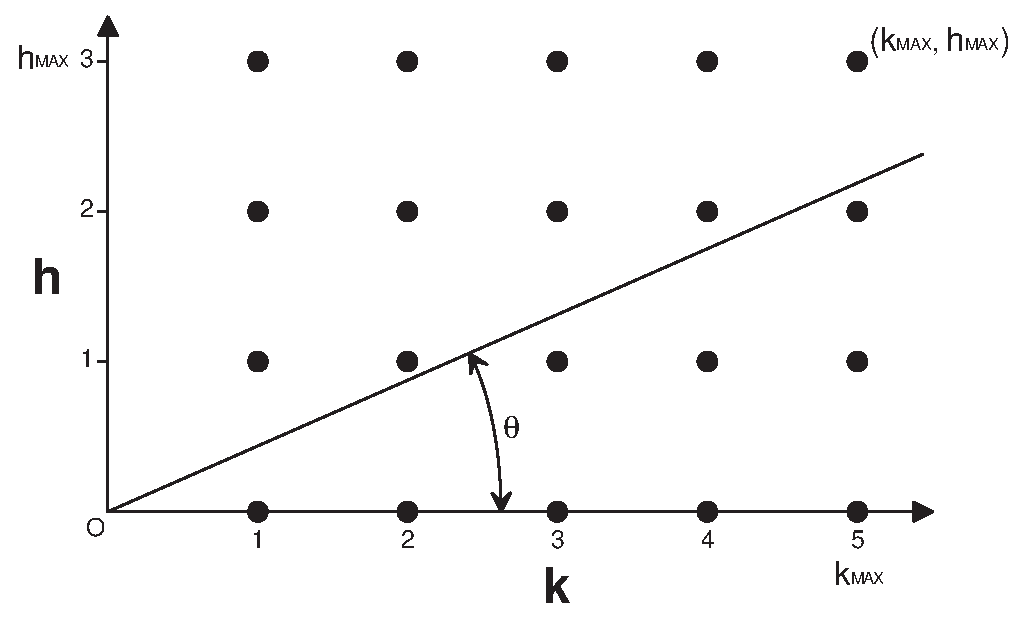
\includegraphics[width=4.25in]{intlat01.eps}
\caption{Integer Lattice Interpretation Of Rational Numbers $h/k$ Formable Under Constraints
        $h \leq h_{MAX}$ And $k \leq k_{MAX}$}
\label{fig:lattice01}
\end{figure}

From Figure \ref{fig:lattice01}, it is clear that:

\begin{generalenum}
\item  The angle $\theta$ of the ray from the origin to $(k,h)$
       is monotonically increasing with respect to the value of
       $h/k$, and:

       \begin{generalenumindent01}
       \item $h/k = tan \theta$.
       \item $\theta = tan^{-1} h/k$.
       \end{generalenumindent01}

\item  The smallest rational number that can be formed under the
       constraints is $0/1$, the smallest non-zero rational number
       is $1/k_{MAX}$, and the largest rational number is $h_{MAX}/1$.

\item  Only irreducible rational numbers are directly ``visible''
       from the origin (reducible numbers are hidden ``behind''
       the irreducible numbers, when viewed from the origin).

\item  The ascending set of irreducible rational numbers that can be formed
       subject to the constraints can be constructed graphically
       by sweeping a line starting at $\theta = 0$ through the range
       $0 \leq \theta < \pi/2$, recording each integer lattice point
       that is directly ``visible'' from the origin.

\item  For $r_A = h/k \leq h_{MAX}/k_{MAX}$, the constraint $k \leq k_{MAX}$ is the
       dominant constraint, and the set of formable rational numbers
       $\leq h_{MAX}/k_{MAX}$ is simply $F_{k_{MAX}}$.

\end{generalenum}

By symmetry in Figure \ref{fig:lattice01}, it can be
seen that each formable rational number $\geq h_{MAX}/k_{MAX}$ is the reciprocal
of an element of the Farey series of order $h_{MAX}$.  Thus, it is clear that
the set of formable rational numbers under the constraints
$h \leq h_{MAX} \wedge k \leq k_{MAX}$ can be built by concatenating
a portion of $F_{k_{MAX}}$ with a portion of $F_{h_{MAX}}$, but with
the terms of $F_{h_{MAX}}$ inverted and reversed in order.

We denote the series formed from $F_N$ by inverting each element (except $0/1$)
and reversing the order as $F_{\overline{N}}$.  For example, using this definition,

\begin{equation}
F_{\overline{3}} =
\left\{
\ldots{},
\frac{3}{8}, \frac{2}{5}, \frac{3}{7},
\frac{1}{2}, \frac{3}{5}, \frac{2}{3}, \frac{3}{4},
\frac{1}{1}, \frac{3}{2}, \frac{2}{1}, \frac{3}{1}
\right\}.
\end{equation}

We denote the series formed by concatenating $F_{k_{MAX}}$ up through
$h_{MAX}/k_{MAX}$ to $F_{\overline{h_{MAX}}}$ from $h_{MAX}/k_{MAX}$
through $h_{MAX}/1$ as $F_{k_{MAX}, \overline{h_{MAX}}}$.

Note that
$F_{k_{MAX}, \overline{h_{MAX}}}$ is the ordered set of all
irreducible rational numbers that can be formed subject to
$h \leq h_{MAX} \wedge k \leq k_{MAX}$.  For example, using this
definition,

\begin{equation}
\label{eq:concatseries01}
F_{5, \overline{3}} =
\left\{
\frac{0}{1}, \frac{1}{5}, \frac{1}{4}, \frac{1}{3},
\frac{2}{5}, \frac{1}{2}, \frac{3}{5},
\frac{2}{3}, \frac{3}{4},
\frac{1}{1}, \frac{3}{2}, \frac{2}{1}, \frac{3}{1}
\right\}.
\end{equation}

It can be verified that the result in (\ref{eq:concatseries01}) is the same
as would be obtained in Figure \ref{fig:lattice01} by sweeping a
line from the origin counterclockwise through $0 \leq \theta < \pi/2$, recording
each point of the integer lattice directly ``visible'' from the origin.

The following $O(log \; max(h_{MAX}, k_{MAX}))$ algorithm is presented
for finding the neighbors in $F_{k_{MAX}, \overline{h_{MAX}}}$ to
an arbitrary irreducible rational number $a/b$.

\begin{algorithm}\label{alg:rectangular}\end{algorithm}
\begin{alglvl0}
\item If $a/b < h_{MAX}/k_{MAX}$, apply Algorithm \ref{alg:bratrnnifnalg}
      directly;
\item Else if $a/b > h_{MAX}/k_{MAX}$, apply Algorithm \ref{alg:bratrnnifnalg}
      using $b/a$, rather than $a/b$ as $r_I$, and using $N=h_{MAX}$ rather than
      $N=k_{MAX}$, and invert and transpose the two
      Farey neighbors obtained;
\item Else if $a/b = h_{MAX}/k_{MAX}$, apply both steps above:  the first step
      to obtain the left neighbor in $F_{k_{MAX}, \overline{h_{MAX}}}$
      and the second step to obtain the right
      neighbor.
\end{alglvl0}


%%%%%%%%%%%%%%%%%%%%%%%%%%%%%%%%%%%%%%%%%%%%%%%%%%%%%%%%%%%%%%%%%%%%%%%%%%%%%%%%%%%%%%%%%%%%%%%%%%%%%%%%
%%%%%%%%%%%%%%%%%%%%%%%%%%%%%%%%%%%%%%%%%%%%%%%%%%%%%%%%%%%%%%%%%%%%%%%%%%%%%%%%%%%%%%%%%%%%%%%%%%%%%%%%
%%%%%%%%%%%%%%%%%%%%%%%%%%%%%%%%%%%%%%%%%%%%%%%%%%%%%%%%%%%%%%%%%%%%%%%%%%%%%%%%%%%%%%%%%%%%%%%%%%%%%%%%
%%%%%%%%%%%%%%%%%%%%%%%%%%%%%%%%%%%%%%%%%%%%%%%%%%%%%%%%%%%%%%%%%%%%%%%%%%%%%%%%%%%%%%%%%%%%%%%%%%%%%%%%
\section{Choosing $r_A = h/k$ Only In An Interval $[l,r]$}
\label{sec:intervalcase}

It is clear from the earlier discussion of the Farey series that the maximum
distance between terms in $F_{k_{MAX}}$ is $1/k_{MAX}$, and that this maximum
distance occurs only adjacent to an integer.  It is also clear from the
discussion of $F_{\overline{h_{MAX}}}$ that the maximum distance between terms
is 1.

Thus, when we use $F_{k_{MAX}, \overline{h_{MAX}}}$ to approximate real numbers,
in general the worst-case distance between terms is 1.

In practical applications when rational approximation is used,
the approximation tends to be used over a restricted interval
$[l \gg  0, r \ll h_{MAX}]$ rather than over the full range of the rational numbers that
can be formed, $[0, h_{MAX}]$.  This section develops novel upper bounds on
the distance between terms of $F_{k_{MAX}, \overline{h_{MAX}}}$ in an interval
$[l,r]$.  For simplicity, assume $l,r \in F_{k_{MAX}, \overline{h_{MAX}}}$.

Three distinct cases are developed (Figure \ref{fig:threecases}).
The upper bound developed from Case III is always larger than the upper
bound developed from Case II, which is always larger than the upper bound developed
from Case I; so if only the absolute maximum error over
the interval $[l,r]$ is of interest, only the
highest-numbered case which applies needs to be evaluated.  However, some
applications may have different error requirements in different regions
of the interval $[l,r]$, and for these applications it may be beneficial
to analyze more than one case.

\begin{figure}
\centering
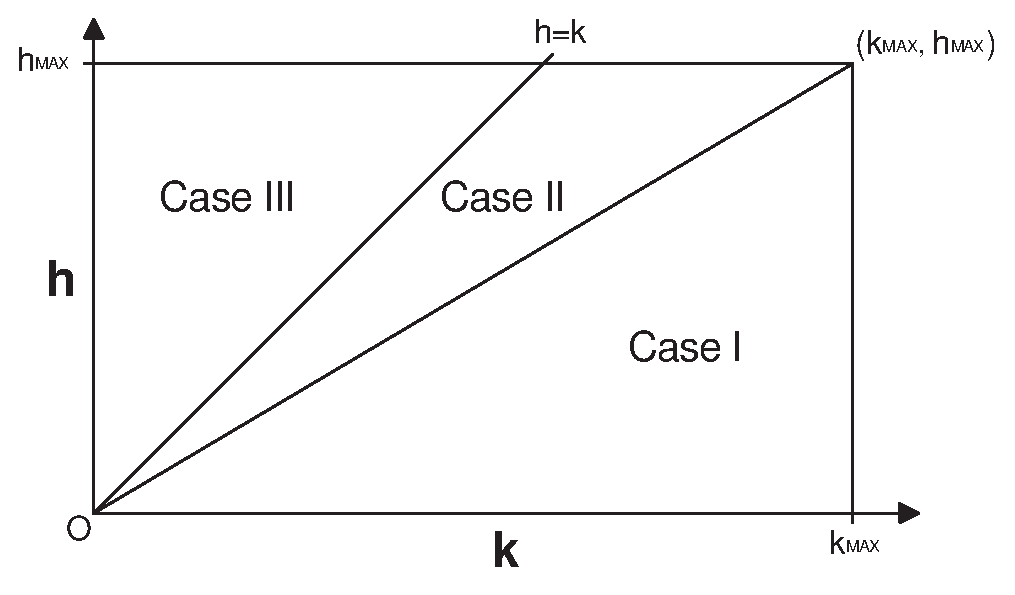
\includegraphics[width=4.25in]{intlat02.eps}
\caption{Three Cases For Bounding Distance Between Terms In $F_{k_{MAX}, \overline{h_{MAX}}}$}
\label{fig:threecases}
\end{figure}


\subsection{Case I:  $r_I < h_{MAX}/k_{MAX}$}
\label{subsec:casei}

With $r_I < h_{MAX}/k_{MAX}$, $k \leq k_{MAX}$ is the dominant
constraint, and the neighbors available to $r_I$ are simply the
terms of $F_{k_{MAX}}$.  If $[l, r] \cap  [0, h_{MAX}/k_{MAX}]$
includes an integer, clearly the maximum distance from $r_I$ to the
nearest available term of $F_{k_{MAX}, \overline{h_{MAX}}}$ is given
by

\begin{equation}
\left|
\frac{h}{k} - r_I
\right|
\leq
\frac{1}{2 k_{MAX}}.
\end{equation}

If $[l, r] \cap  [0, h_{MAX}/k_{MAX}]$ does
not include an integer, it can be shown that the
maximum distance between Farey terms is driven by the
rational number with the smallest denominator in the
interval.

For two consecutive terms $p/q$ and $p'/q'$ in $F_{k_{MAX}}$,
$p'q - pq' = 1$ (Theorem \ref{thm:thm01}), so that

\begin{equation}
\frac{p'}{q'} - \frac{p}{q} =
\frac{p'q - pq'}{q q'} = \frac{1}{qq'} .
\end{equation}

By Theorem \ref{thm:thm03}, $q+q' > k_{MAX}$, therefore

\begin{equation}
\label{eq:minqplacementupperbound}
\frac{1}{q k_{MAX}} \leq
\frac{1}{q q'} <
\frac{1}{q (k_{MAX}-q)}.
\end{equation}

Let $q_{MIN}$ be the smallest denominator of any rational number
$\in F_{k_{MAX}}$ in the interval $[l,r]$.  It is then easy to show
that for any consecutive denominators $q, q'$ which occur in
$F_{k_{MAX}}$ in the interval $[l,r]$,

\begin{equation}
\frac{1}{q q'} < \frac{1}{q_{MIN} \; max (q_{MIN}, k_{MAX} - q_{MIN})} .
\end{equation}

Thus, the upper bound on the distance between consecutive terms of $F_{k_{MAX}}$
in an interval $[l,r]$ is tied to the minimum denominator of any
rational number $\in F_{k_{MAX}}$ in $[l,r]$.

Note that clearly
$q_{MIN} \leq 1/(r-l)$, so for most practical intervals $[l,r]$,
the search for $q_{MIN}$ would not be computationally expensive.
However, applications could arise where an approximation is used
in an \emph{extremely} narrow interval, and having an algorithm available that
is computationally viable for such cases is advantageous.  For example,
locating the rational number $\in F_{2^{20,000}}$ with the smallest denominator
in an interval of width $2^{-10,000}$ could be a serious computational
problem.

To locate $q_{MIN}$ in $[l,r]$, note that at least one rational number
with $q_{MIN}$ as a denominator in $[l,r]$ is the best approximation
of order $q_{MIN}$ to the midpoint of the interval,
$(l+r)/2$.\footnote{Thanks to David M. Einstein and David Eppstein
for this observation, contributed via the \texttt{sci.math} newsgroup,
which is the linchpin of Algorithm \ref{alg:cfmindenominator}.}
By theorem (\cite{KhinchinClassic}, Theorem 15), every best approximation
of a number is a convergent or intermediate fraction of the
continued fraction representation of the number.  We seek the
convergent or intermediate fraction of $(l+r)/2$ with the smallest
denominator that is in the interval $[l,r]$.

The convergents and intermediate fractions of $(l+r)/2$ are naturally
arranged in order of increasing denominator.  However, it would be
inefficient to test \emph{every} intermediate fraction
for membership in $[l,r]$, as partial quotients $a_k$ are unlimited in
size and such an algorithm may not be $O(log \; k_{MAX})$.  Instead,
since intermediate fractions are formed using the parameterized
expression $(i p_k + p_{k-1})/(i q_k + q_{k-1})$,
and since intermediate fractions are ever-increasing
or ever-decreasing with respect to the parameter $i$, the
smallest value of $i$ which will create an intermediate
fraction potentially within $[l,r]$ can be directly
calculated.  Only the intermediate fraction formed with
this calculated value of $i$ needs to be tested for membership in
$[l,r]$.

Let $l_N$ and $l_D$ be the numerator and denominator of $l$, and
let $r_N$ and $r_D$ be the numerator and denominator of $r$.
In the case of $k$ even; $s_k < l < (l+r)/2$ (otherwise $s_k$
would have been identified as $\in [l,r]$, see Algorithm
\ref{alg:cfmindenominator}); $s_{k+1} \geq (l+r)/2$;
with increasing $i$, $(i p_k + p_{k-1})/(i q_k + q_{k-1})$
forms a decreasing sequence; and the inequality we seek to solve is

\begin{equation}
\label{eq:ifselection01}
\frac{i p_k + p_{k-1}}{i q_k + q_{k-1}} \leq \frac{r_N}{r_D}.
\end{equation}

Solving (\ref{eq:ifselection01}), the smallest integral value of $i$ that will suffice is

\begin{equation}
\label{eq:ifselection02}
i = \left\lceil {
\frac{r_N q_{k-1} - r_D p_{k-1}}{r_D p_k - r_N q_k}
} \right\rceil .
\end{equation}

Similarly, for $k$ odd, the sequence is increasing,
and the inequality and solution are

\begin{equation}
\label{eq:ifselection03}
\frac{i p_k + p_{k-1}}{i q_k + q_{k-1}} \geq \frac{l_N}{l_D}
\to
i = \left\lceil {
\frac{l_N q_{k-1} - l_D p_{k-1}}{l_D p_k - l_N q_k}
} \right\rceil .
\end{equation}

(\ref{eq:ifselection01}),
(\ref{eq:ifselection02}),
and (\ref{eq:ifselection03}) suggest the following continued fraction
algorithm for finding
a rational number with the smallest denominator in an
interval $[l,r]$.

\begin{algorithm}\label{alg:cfmindenominator}\end{algorithm}
\begin{alglvl0}
\item Calculate all partial quotients $a_k$ and all convergents
      $s_k = p_k/q_k$ of the midpoint of the interval,
      $(l+r)/2$.

\item  For each convergent $s_k=p_k/q_k$, in order of increasing $k$:

   \begin{alglvl1}

   \item If $s_k = p_k/q_k \in [l,r]$, $s_k$ is a rational number with
         the lowest denominator, STOP.

   \item If $k$ is even,

      \begin{alglvl2}

      \item Calculate $i$ according to (\ref{eq:ifselection02}).
            If $i < a_{k+1}$ and the intermediate fraction
            $(i p_k + p_{k-1})$ $/$ $(i q_k + q_{k-1})$ $\geq$ $l$, this intermediate
            fraction is
            a rational number with the lowest denominator, STOP.

      \end{alglvl2}

   \item Else if $k$ is odd,

      \begin{alglvl2}

      \item Calculate $i$ according to (\ref{eq:ifselection03}).
            If $i < a_{k+1}$ and the intermediate fraction
            $(i p_k + p_{k-1})$ $/$ $(i q_k + q_{k-1})$ $\leq$ $r$, this intermediate
            fraction is
            a rational number with the lowest denominator, STOP.

      \end{alglvl2}

   \end{alglvl1}

\end{alglvl0}

Algorithm \ref{alg:cfmindenominator} is approximately $O(log \; k_{MAX})$,
since there are a fixed number of steps per convergent, and the maximum number
of convergents is $O(log \; k_{MAX})$.  Once a rational number with the smallest
denominator $q_{MIN}$ is located, (\ref{eq:minqplacementupperbound})
can be applied to bound $|r_A - r_I|$; namely,

\begin{equation}
\label{eq:qminmaxplacementerror}
\left| {\frac{h}{k} - r_I}  \right|
<
\frac{1}{2q_{MIN} \; max(q_{MIN}, k_{MAX} - q_{MIN})} .
\end{equation}


\subsection{Case II:  $h_{MAX}/k_{MAX} < r_I < 1$}
\label{subsec:caseii}

If $h_{MAX}/k_{MAX} < r_I < 1$, a graphical argument
(Figure \ref{fig:caseii}) can be used
to more tightly bound the maximum distance between terms of
$F_{k_{MAX}, \overline{h_{MAX}}}$.

\begin{figure}
\centering
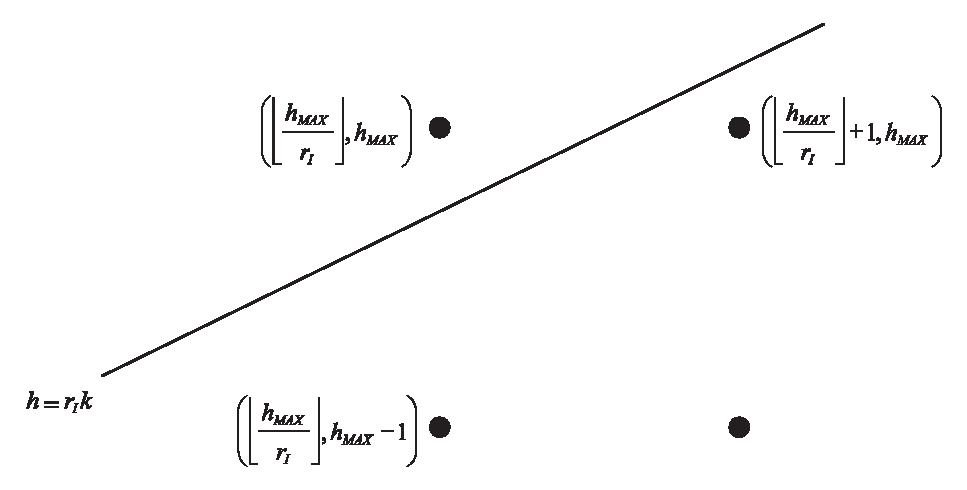
\includegraphics[height=2.0in]{intlat03.eps}
\caption{Graphical Interpretation Of Case II:  $h_{MAX}/k_{MAX} < r_I < 1$}
\label{fig:caseii}
\end{figure}

In this case,  a formable term at or to the left\footnote{To the left on the
number line, but to the right in Figure \ref{fig:caseii}.}
of $r_I$ is represented by the point $(\lfloor h_{MAX}/r_I \rfloor + 1, h_{MAX} )$
in the integer lattice,
and a formable term at or to the right of $r_I$ is
represented by the point $(\lfloor h_{MAX}/r_I \rfloor, h_{MAX} )$
in the integer lattice.  Thus, the maximum distance between
neighboring terms in $F_{k_{MAX}, \overline{h_{MAX}}}$
is given by the difference of these two terms,

\begin{equation}
\frac{h_{MAX}}{\left\lfloor {\frac{h_{MAX}}{r_I}} \right\rfloor}
-
\frac{h_{MAX}}{\left\lfloor {\frac{h_{MAX}}{r_I}} \right\rfloor + 1}
=
\frac{h_{MAX}}{{\left\lfloor {\frac{h_{MAX}}{r_I}} \right\rfloor}^2
+ \left\lfloor {\frac{h_{MAX}}{r_I}} \right\rfloor},
\end{equation}

and the maximum distance from $r_I$ to a neighboring term is
given by

\begin{equation}
\label{eq:caseiimaxplacementerror}
\left|
\frac{h}{k} - r_I
\right|
\leq
\frac{h_{MAX}}{2 \left( { {\left\lfloor {\frac{h_{MAX}}{r_I}} \right\rfloor}^2
+ \left\lfloor {\frac{h_{MAX}}{r_I}} \right\rfloor } \right) }.
\end{equation}

Note that Case II will exist only if $h_{MAX}/k_{MAX} < 1$.


\subsection{Case III:  $1 < h_{MAX}/k_{MAX} < r_I$}
\label{subsec:caseiii}

It can be established graphically, using the coordinate system of
Figure \ref{fig:lattice01}
or Figure \ref{fig:threecases}, that the line $h=r_I k$ intercepts the
line $h=h_{MAX}$ at the point $(h_{MAX}/r_I, h_{MAX})$.  It is clear
from a graphical argument that all of the terms of the Farey series
of order $\lfloor h_{MAX}/r_I \rfloor$ are available as neighbors
of $r_I$.  Therefore,

\begin{equation}
\label{caseiiiplacementerror}
\left|
\frac{h}{k} - r_I
\right|
\leq
\frac{1}{2 \left\lfloor \frac{h_{MAX}}{r_I} \right\rfloor}.
\end{equation}


%%%%%%%%%%%%%%%%%%%%%%%%%%%%%%%%%%%%%%%%%%%%%%%%%%%%%%%%%%%%%%%%%%%%%%%%%%%%%%%%%%%%%%%%%%%%%%%%%%%%%%%%
%%%%%%%%%%%%%%%%%%%%%%%%%%%%%%%%%%%%%%%%%%%%%%%%%%%%%%%%%%%%%%%%%%%%%%%%%%%%%%%%%%%%%%%%%%%%%%%%%%%%%%%%
%%%%%%%%%%%%%%%%%%%%%%%%%%%%%%%%%%%%%%%%%%%%%%%%%%%%%%%%%%%%%%%%%%%%%%%%%%%%%%%%%%%%%%%%%%%%%%%%%%%%%%%%
%%%%%%%%%%%%%%%%%%%%%%%%%%%%%%%%%%%%%%%%%%%%%%%%%%%%%%%%%%%%%%%%%%%%%%%%%%%%%%%%%%%%%%%%%%%%%%%%%%%%%%%%
\section{End-To-End Approximation Error}
\label{sec:endtoenderror}

A rational approximation requires an integer domain and range, and there are three
sources of error inherent in such an approximation:

\begin{generalenum}

\item Input quantization error, as the input to the approximation is restricted
      to $\intsetnonneg$.

\item Error in selecting $r_A = h / k$, as in general it isn't possible to choose
      $r_A = r_I$.

\item Output quantization error, as the remainder of the division of $hx$ by
      $k$ is discarded, and the output must be $\in \intsetnonneg$.

\end{generalenum}

To model the end-to-end approximation error, a model function
is introduced which represents the function we wish to approximate,

\begin{equation}
\label{eq:eq0001}
F(x)=r_{I}x .
\end{equation}

However, the approximation necessarily involves quantizing
the input $x$, as well as the result of the integer division:

\begin{equation}
\label{eq:eq0006}
J(x) = \left\lfloor {r_A \left\lfloor x \right\rfloor } \right\rfloor
   = \left\lfloor {\frac{{h\left\lfloor x \right\rfloor }}{k}} \right\rfloor .
\end{equation}

Quantization of a real argument $x$ which is not necessarily
rational is treated by noting that quntization introduces an
error $\varepsilon \in [0,1)$:

\begin{equation}
\lfloor x \rfloor = x - \varepsilon; \; \varepsilon \in [0,1) .
\end{equation}

Quantization of a rational argument $a/b$ is treated
by noting that the largest quantization error $\varepsilon$
occurs when $a$ is one less than an integral multiple of
$b$:

\begin{equation}
\left\lfloor {\frac{a}{b}} \right\rfloor
=
\frac{a}{b} - \varepsilon; \;
\varepsilon \in
\left[ {0, \frac{b-1}{b}} \right] .
\end{equation}

The difference function $J(x)-F(x)$, can be stated
as in (\ref{eq:eq0031}) or (\ref{eq:eq0032}).  The two quantizations in (\ref{eq:eq0031})
can be treated by introducing $\varepsilon_{1}$
and $\varepsilon_{2}$ to yield (\ref{eq:eq0032}).
Note that $\varepsilon_{1}$ and $\varepsilon_{2}$
are independent, meaning for this application that in general $r_I$,
$r_A = h/k$, and $x$ can be
chosen so as to force any combination of $\varepsilon_{1}$ and
$\varepsilon_{2}$, so that no combinations of $\varepsilon_{1}$ and $\varepsilon_{2}$
can be excluded.

\begin{equation}
\label{eq:eq0031}
J(x) - F(x) = \left\lfloor {\frac{{h\left\lfloor x \right\rfloor
     }}{k}} \right\rfloor  - r_I x
\end{equation}

\begin{equation}
\label{eq:eq0032}
J(x) - F(x) = \frac{{h(x - \varepsilon _1 ) }}{k} - \varepsilon _2  - r_I x
; \;
\varepsilon _1  \in [0,1)
; \;
\varepsilon _2  \in \left[ {0,\frac{{k - 1}}{k}} \right]
\end{equation}

Choosing the extremes of
$\varepsilon_{1}$ and $\varepsilon_{2}$
so as to minimize and maximize the difference
function bounds the approximation error (\ref{eq:eq0035}).

\begin{equation}
\label{eq:eq0035}
  J(x) - F(x) \in
  \left( {(r_A  - r_I )x - r_A  - \frac{{k - 1}}{k},(r_A  - r_I )x } \right]
\end{equation}

Minimizing and maximizing (\ref{eq:eq0035}) over
a domain of $[0,x_{MAX}]$ leads to (\ref{eq:eq0036}).

\begin{equation}
\label{eq:eq0036}
  \left. {J(x) - F(x)} \right|_{x \in [0,x_{MAX} ]}  \in
  \left\{ {\begin{array}{*{20}c}
   {\left( {(r_A  - r_I )x_{MAX}  - r_A  - \frac{{k - 1}}{k},0} \right],}
    \hfill & {r_A  < r_I } \hfill  \\
   \\
   {\left( { - r_A  - \frac{{k - 1}}{k},0} \right],} \hfill & {r_A  = r_I } \hfill  \\
   \\
   {\left( { - r_A  - \frac{{k - 1}}{k},(r_A  - r_I )x_{MAX} } \right] ,}
    \hfill & {r_A  > r_I } \hfill  \\
\end{array}} \right.
\end{equation}

Thus, given an $r_I \in \realsetnonneg$ and a rational approximation to $r_I$,
$r_A = h/k$, the error introduced by this rational approximation used over a
domain $[0,x_{MAX}]$ can be bounded.


%%%%%%%%%%%%%%%%%%%%%%%%%%%%%%%%%%%%%%%%%%%%%%%%%%%%%%%%%%%%%%%%%%%%%%%%%%%%%%%%%%%%%%%%%%%%%%%%%%%%%%%%
%%%%%%%%%%%%%%%%%%%%%%%%%%%%%%%%%%%%%%%%%%%%%%%%%%%%%%%%%%%%%%%%%%%%%%%%%%%%%%%%%%%%%%%%%%%%%%%%%%%%%%%%
%%%%%%%%%%%%%%%%%%%%%%%%%%%%%%%%%%%%%%%%%%%%%%%%%%%%%%%%%%%%%%%%%%%%%%%%%%%%%%%%%%%%%%%%%%%%%%%%%%%%%%%%
%%%%%%%%%%%%%%%%%%%%%%%%%%%%%%%%%%%%%%%%%%%%%%%%%%%%%%%%%%%%%%%%%%%%%%%%%%%%%%%%%%%%%%%%%%%%%%%%%%%%%%%%
\section{Design Example}
\label{sec:designexample}

A design example is presented to illustrate the methods presented.
An $r_I$ specified with only modest precision and an
$h_{MAX}$ and $k_{MAX}$ of only modest size are used to avoid a large
number of partial quotients or large integers.\footnote{The rational
approximation
software submitted with this paper will handle rational approximations involving hundreds
of digits and hundreds of partial quotients.  However, such approximations make unsuitable
examples because of the length, the difficulty in typesetting huge integers and
rational numbers, and because
the examples can't be carried out manually by a reader.}

\textbf{Design Example:}
Assume that real numbers are to be approximated by rational numbers
in the interval $[0.385, 2.160]$, subject to $h_{MAX} = 193 \wedge k_{MAX}=500$.
Bound $|r_A - r_I|$ under these constraints.  Find the best rational
approximations to $1/\pi \approx 0.31830989$ and
$2/\pi \approx 0.63661977$ under the same constraints.

\textbf{Solution:}
In this example, \emph{Case I}, \emph{Case II}, and \emph{Case III}
(Sections \ref{subsec:casei}, \ref{subsec:caseii}, and \ref{subsec:caseiii}) apply.  Case III
will dominate the upper bound on the error in selecting $r_A$,
but it is instructive to work through Case I and Case II.

To apply the results from \emph{Case I}, it is necessary to find
a rational number with the smallest denominator in the interval
$[l = 0.385, r = 193/500 = 0.386]$.  The midpoint of the interval
is $(l+r)/2 = 0.3855 = 771/2000$.

Table \ref{tbl:cfexpansmidpoint} shows the generation of the partial quotients and convergents of the
midpoint, 771/2000, using Algorithm \ref{alg:bratrnnifnalg}.

\begin{table}
\caption{Partial Quotients And Convergents Of 0.3855 (Midpoint Of The Interval
        $[0.385, 0.386]$)}
\label{tbl:cfexpansmidpoint}
\begin{center}
\begin{tabular}{|c|c|c|c|c|c|c|}
\hline
\small{Index} & \small{$dividend_k$}  & \small{$divisor_k$} & \small{$a_k$}   & \small{$remainder_k$} & \small{$p_k$}      & \small{$q_k$}       \\
\small{($k$)} &                       &                     &                 &                       &                    &                     \\
\hline
\hline
\small{-1}    & \small{N/A}           & \small{771}         & \small{N/A}     & \small{2000}          & \small{1}          & \small{0}           \\
\hline
\small{0}     & \small{771}           & \small{2000}        & \small{0}       & \small{771}           & \small{0}          & \small{1}           \\
\hline
\small{1}     & \small{2000}          & \small{771}         & \small{2}       & \small{458}           & \small{1}          & \small{2}           \\
\hline
\small{2}     & \small{771}           & \small{458}         & \small{1}       & \small{313}           & \small{1}          & \small{3}           \\
\hline
\small{3}     & \small{458}           & \small{313}         & \small{1}       & \small{145}           & \small{2}          & \small{5}           \\
\hline
\small{4}     & \small{313}           & \small{145}         & \small{2}       & \small{23}            & \small{5}          & \small{13}          \\
\hline
\small{5}     & \small{145}           & \small{23}          & \small{6}       & \small{7}             & \small{32}         & \small{83}          \\
\hline
\small{6}     & \small{23}            & \small{7}           & \small{3}       & \small{2}             & \small{101}        & \small{262}         \\
\hline
\small{7}     & \small{7}             & \small{2}           & \small{3}       & \small{1}             & \small{335}        & \small{869}         \\
\hline
\small{8}     & \small{2}             & \small{1}           & \small{2}       & \small{0}             & \small{771}        & \small{2000}        \\
\hline
\end{tabular}
\end{center}
\end{table}

Algorithm \ref{alg:cfmindenominator} can be applied to locate the fraction
in $[l,r]$ with the smallest denominator.  $s_0 =0/1 \notin [l,r]$.  The intermediate fraction
$(p_0 + p_{-1})/(q_0 + q_{-1})=1/1 \notin [l,r]$. $s_1 = 1/2 \notin [l,r]$.
$s_2 = 1/3 \notin [l,r]$.  $s_3 = 2/5 \notin [l,r]$.  The intermediate fraction
$(p_3 + p_2)/(q_3 + q_2)=3/8 \notin [l,r]$.  $s_4 = 5/13 \notin [l,r]$.
(\ref{eq:ifselection02}) can be applied to determine the lowest value of the
parameter $i$ for which an intermediate fraction \emph{may} be in $[l,r]$:

\begin{equation}
i = \left\lceil {
\frac
{(r_N = 193)(q_3 = 5) - (r_D = 500)(p_3=2)}
{(r_D=500)(p_4 = 5)-(r_N=193)(q_4=13)}
} \right\rceil
=
\left\lceil {\frac{-35}{-9}} \right\rceil = 4.
\end{equation}

Thus, it is only necessary to examine the intermediate fraction $(4 p_4 + p_3)/(4 q_4 + q_3)$
for potential membership in $[l,r]$.  This intermediate fraction, $22/57$ $\approx$ $0.385965$ $\in$ $[l,r]$.
Thus, the fraction with the lowest denominator in the interval is 22/57, and $q_{min} = 57$.

Application of (\ref{eq:qminmaxplacementerror}) yields

\begin{equation}
\begin{array}{l}
\displaystyle{\left| {\frac{h}{k} - r_I} \right| < } \\
\\
\displaystyle{\left({\frac{1}{2q_{MIN} \; max(q_{MIN}, k_{MAX}-q_{MIN})} = \frac{1}{(2)(57)(500-57)} = \frac{1}{50,502} } \right) .}
\end{array}
\end{equation}

Note that the 1/50,502 maximum error in placing $r_A$ is much better than the
1/1,000 worst-case error for $F_{500}$ in general without restrictions on
the interval.

Case II and Case III aren't as complicated as Case I---applying these
cases is a simple matter of substitution into (\ref{eq:caseiimaxplacementerror})
or (\ref{caseiiiplacementerror}).
Case II and
(\ref{eq:caseiimaxplacementerror}) apply, but the error bounds from
Case III will be larger, so Case II is not evaluated.
Case III applies: the line $h=r_I k$ intersects the line $h=h_{MAX}$ at
the point
$(h_{MAX}/r_I, h_{MAX})$ = $(193/2.160, 193)$, thus all terms
of the Farey series of order $\lfloor 193/2.160 \rfloor = 89$ are
available for selection.  Therefore, applying (\ref{caseiiiplacementerror}),

\begin{equation}
\left| {\frac{h}{k} - r_I} \right|
\leq
\frac{1}{2 \times 89} \approx 0.0056 .
\end{equation}

Thus, if $F_{500, \overline{193}}$ is used to approximate real numbers over the
interval $[0.385$, $2.160]$, an upper bound on $|r_A - r_I|$ is $1/178 \approx 0.0056$.
Note that Case III dominates, and that the upper bound on $|r_A - r_I|$ varies
within the interval.

To find the best rational approximations to $1/ \pi$ in $F_{500, \overline{193}}$,
note that $1/ \pi < 193/500$, so all of the terms in $F_{500}$ are available.
Table \ref{tbl:cfexpansraponeoverpi} shows the partial quotients and convergents
of $1/ \pi$, using 0.31830989 as a rational approximation of $1/ \pi$.  $s_4$
is the highest-order convergent with $q_k \leq 500$, so $s_4 = 113/355$ is one
Farey neighbor to $1/ \pi$ in $F_{500}$.  Applying (\ref{eq:eq0065}) to generate
the other neighbor in $F_{500}$ yields 106/333.  Note that $113/355 - 1/\pi \approx -3 \times 10^{-8}$
and $106/333 - 1/\pi \approx 8 \times 10^{-6}$ (the errors are quite small).

\begin{table}
\caption{Partial Quotients And Convergents Of 31,830,989/100,000,000
        (A Rational Approximation To $1/ \pi$)}
\label{tbl:cfexpansraponeoverpi}
\begin{center}
\begin{tabular}{|c|c|c|c|c|c|c|}
\hline
\small{Index} & \small{$dividend_k$}  & \small{$divisor_k$} & \small{$a_k$}   & \small{$remainder_k$} & \small{$p_k$}      & \small{$q_k$}       \\
\small{($k$)} &                       &                     &                 &                       &                    &                     \\
\hline
\hline
\small{-1}    & \small{N/A}           & \small{31,830,989}  & \small{N/A}     & \small{100,000,000}   & \small{1}          & \small{0}           \\
\hline
\small{0}     & \small{31,830,989}    & \small{100,000,000} & \small{0}       & \small{31,830,989}    & \small{0}          & \small{1}           \\
\hline
\small{1}     & \small{100,000,000}   & \small{31,830,989}  & \small{3}       & \small{4,507,033}     & \small{1}          & \small{3}           \\
\hline
\small{2}     & \small{31,830,989}    & \small{4,507,033}   & \small{7}       & \small{281,758}       & \small{7}          & \small{22}          \\
\hline
\small{3}     & \small{4,507,033}     & \small{281,758}     & \small{15}      & \small{280,663}       & \small{106}        & \small{333}         \\
\hline
\small{4}     & \small{281,758}       & \small{280,663}     & \small{1}       & \small{1,095}         & \small{113}        & \small{355}         \\
\hline
\small{5}     & \small{280,663}       & \small{1,095}       & \small{256}     & \small{343}           & \small{29,034}     & \small{91,213}      \\
\hline
\small{6}     & \small{1,095}         & \small{343}         & \small{3}       & \small{66}            & \small{87,215}     & \small{273,994}     \\
\hline
\small{7}     & \small{343}           & \small{66}          & \small{5}       & \small{13}            & \small{465,109}    & \small{1,461,183}   \\
\hline
\small{8}     & \small{66}            & \small{13}          & \small{5}       & \small{1}             & \small{2,412,760}  & \small{7,579,909}   \\
\hline
\small{9}     & \small{13}            & \small{1}           & \small{13}      & \small{0}             & \small{31,830,989} & \small{100,000,000} \\
\hline
\end{tabular}
\end{center}
\end{table}

To find the best rational approximations to $2/ \pi$ in $F_{500, \overline{193}}$,
note that $2/ \pi > 193/500$, so the second clause of Algorithm \ref{alg:rectangular}
applies.  Table \ref{tbl:cfexpansrappiovertwo} shows the partial quotients and convergents
of $\pi / 2$, using 1/0.63661977 as a rational approximation of $\pi /2$.  $s_3$
is the highest-order convergent with $q_k \leq 193$, so $s_3^{-1} = (11/7)^{-1}$ is one
neighbor to $2/ \pi$ in $F_{\overline{193}}$.  Applying (\ref{eq:eq0065}) to generate
the reciprocal of the other neighbor in $F_{\overline{193}}$ yields 300/191, implying that
191/300 is the other neighbor.  $7/11 - 2/\pi \approx -3 \times 10^{-4}$.
$191/300 - 2/\pi \approx 5 \times 10^{-5}$.

\begin{table}
\caption{Partial Quotients And Convergents Of 100,000,000/63,661,977
        (A Rational Approximation To $\pi / 2$)}
\label{tbl:cfexpansrappiovertwo}
\begin{center}
\begin{tabular}{|c|c|c|c|c|c|c|}
\hline
\small{Index} & \small{$dividend_k$}  & \small{$divisor_k$} & \small{$a_k$}   & \small{$remainder_k$} & \small{$p_k$}      & \small{$q_k$}       \\
\small{($k$)} &                       &                     &                 &                       &                    &                     \\
\hline
\hline
\small{-1}    & \small{N/A}           & \small{100,000,000} & \small{N/A}     & \small{63,661,977}    & \small{1}          & \small{0}           \\
\hline
\small{0}     & \small{100,000,000}   & \small{63,661,977}  & \small{1}       & \small{36,338,023}    & \small{1}          & \small{1}           \\
\hline
\small{1}     & \small{63,661,977}    & \small{36,338,023}  & \small{1}       & \small{27,323,954}    & \small{2}          & \small{1}           \\
\hline
\small{2}     & \small{36,338,023}    & \small{27,323,954}  & \small{1}       & \small{9,014,069}     & \small{3}          & \small{2}           \\
\hline
\small{3}     & \small{27,323,954}    & \small{9,014,069}   & \small{3}       & \small{281,747}       & \small{11}         & \small{7}           \\
\hline
\small{4}     & \small{9,014,069}     & \small{281,747}     & \small{31}      & \small{279,912}       & \small{344}        & \small{219}         \\
\hline
\small{5}     & \small{281,747}       & \small{279,912}     & \small{1}       & \small{1,835}         & \small{355}        & \small{226}         \\
\hline
\small{6}     & \small{279,912}       & \small{1,835}       & \small{152}     & \small{992}           & \small{54,304}     & \small{34,571}      \\
\hline
\small{7}     & \small{1,835}         & \small{992}         & \small{1}       & \small{843}           & \small{54,659}     & \small{34,797}      \\
\hline
\small{8}     & \small{992}           & \small{843}         & \small{1}       & \small{149}           & \small{108,963}    & \small{69,368}      \\
\hline
\small{9}     & \small{843}           & \small{149}         & \small{5}       & \small{98}            & \small{599,474}    & \small{381,637}     \\
\hline
\small{10}    & \small{149}           & \small{98}          & \small{1}       & \small{51}            & \small{708,437}    & \small{451,005}     \\
\hline
\small{11}    & \small{98}            & \small{51}          & \small{1}       & \small{47}            & \small{1,307,911}  & \small{832,642}     \\
\hline
\small{12}    & \small{51}            & \small{47}          & \small{1}       & \small{4}             & \small{2,016,348}  & \small{1,283,647}   \\
\hline
\small{13}    & \small{47}            & \small{4}           & \small{11}      & \small{3}             & \small{23,487,739} & \small{14,952,759}  \\
\hline
\small{14}    & \small{4}             & \small{3}           & \small{1}       & \small{1}             & \small{25,504,087} & \small{16,236,406}  \\
\hline
\small{15}    & \small{3}             & \small{1}           & \small{3}       & \small{0}             & \small{100,000,000}& \small{63,661,977}  \\
\hline
\end{tabular}
\end{center}
\end{table}


%%%%%%%%%%%%%%%%%%%%%%%%%%%%%%%%%%%%%%%%%%%%%%%%%%%%%%%%%%%%%%%%%%%%%%%%%%%%%%%%%%%%%%%%%%%%%%%%%%%%%%%%%
%%%%%%%%%%%%%%%%%%%%%%%%%%%%%%%%%%%%%%%%%%%%%%%%%%%%%%%%%%%%%%%%%%%%%%%%%%%%%%%%%%%%%%%%%%%%%%%%%%%%%%%%%
%% (9) ACKNOWLEDGEMENTS                                                                                 %
%%%%%%%%%%%%%%%%%%%%%%%%%%%%%%%%%%%%%%%%%%%%%%%%%%%%%%%%%%%%%%%%%%%%%%%%%%%%%%%%%%%%%%%%%%%%%%%%%%%%%%%%%
%%%%%%%%%%%%%%%%%%%%%%%%%%%%%%%%%%%%%%%%%%%%%%%%%%%%%%%%%%%%%%%%%%%%%%%%%%%%%%%%%%%%%%%%%%%%%%%%%%%%%%%%%
%%Need to retain e-mail addresses to contact all people who have contributed
%%to thank.
%%Greg Bachelis (greg@math.wayne.edu)
%%Robert Berman (rberman@math.wayne.edu)
%%Feng Lin (flin@ece.eng.wayne.edu)
%%Nick Sahinidis (nikos@uiuc.edu)
%%Adam Van Tuyl, (vantuyl@mast.queensu.ca)
%%Carl Schweiger (carl@titan.princeton.edu)
%%Ken Tindell (ktindell@ssx5.com)
%%Steve Vestal (vestal@htc.honeywell.com)
%%Bob Whitinger (bob@whitinger.net, bob.whitinger@sea.siemens.com)
%%David B. Stewart (dstewart@eng.umd.edu)
%%Johan Bengtsson (johanb@docs.uu.se)
%%Michael J. Burke (mburke@visteon.com)
%%Mark Endicott (mendicot@visteon.com)
%%David Eppstein (eppstein@ics.uci.edu)
%%Cliff Stallings (cliff@eng.wayne.edu)
%%Robert Kakos (robert@enterprise.eng.wayne.edu)
%%Klaus-Peter Zauner (kjz@cs.wayne.edu)
%%Karsten Tinnefeld (tinnefeld@ls2.cs.uni-dortmund.de)
%%Paulette Groen (pgroen@visteon.com)
%%Paula Smith (psmith77@visteon.com)
%%Mircea Munteanu (mmuntean@visteon.com)
%%Adam Gibson (adam.g@virgin.net)
%%Virgil (vmhjr@frii.com)
%%Bob Crosby (b-crosby@ti.com)
%%Una Smith (una.smith@yale.edu)
%%Andrea Blome (ablome@mail.cfigroup.com)
%%Axel Franke (Axel.Franke@physics.umu.se)
%%
%%Need also to include Adam's Web site on my Web page,
%%http://archives.math.utk.edu/articles/atuyl/confrac/
%%
%%Need also to include David Eppstein's Web site
%%http://www.ics.uci.edu/~eppstein/
%%
%%
\begin{acks}
We would like to gratefully acknowledge the assistance
of Greg Bachelis, Robert Berman, Feng
Lin, Nick Sahinidis, Adam Van Tuyl,
Carl Schweiger, Ken Tindell, Steve Vestal,
Bob Whitinger, and David B. Stewart
in finding the areas of
mathematics relevant to the rational number selection
problem.  We would also like to
thank Johan Bengtsson, Michael J. Burke,
Mark Endicott, David Eppstein,
David M. Einstein, Mircea Munteanu,
Adam Gibson, and Virgil (of the \texttt{sci.math.num-analysis} newsgroup)
for insight into this problem; Cliff Stallings and
Robert Kakos for support from Wayne State
University's College Of Engineering; Paulette Groen and
Paula Smith for support from Visteon; Bob Crosby for support
from Texas Instruments; Klaus-Peter Zauner, Andrea Blome,
Una Smith, Karsten Tinnefeld, and
Axel Franke for other tool
and logistical support; and the management
team at Visteon for allowing us to pursue this
effort in the workplace.
\end{acks}

%%%%%%%%%%%%%%%%%%%%%%%%%%%%%%%%%%%%%%%%%%%%%%%%%%%%%%%%%%%%%%%%%%%%%%%%%%%%%%%%%%%%%%%%%%%%%%%%%%%%%%%%%
%%%%%%%%%%%%%%%%%%%%%%%%%%%%%%%%%%%%%%%%%%%%%%%%%%%%%%%%%%%%%%%%%%%%%%%%%%%%%%%%%%%%%%%%%%%%%%%%%%%%%%%%%
%% (11) REFERENCES                                                                                      %
%%%%%%%%%%%%%%%%%%%%%%%%%%%%%%%%%%%%%%%%%%%%%%%%%%%%%%%%%%%%%%%%%%%%%%%%%%%%%%%%%%%%%%%%%%%%%%%%%%%%%%%%%
%%%%%%%%%%%%%%%%%%%%%%%%%%%%%%%%%%%%%%%%%%%%%%%%%%%%%%%%%%%%%%%%%%%%%%%%%%%%%%%%%%%%%%%%%%%%%%%%%%%%%%%%%
\nocite{*}
\bibliographystyle{ESUB2ACM}
\begin{thebibliography}{1}

\bibitem{HardyAndWrightClassic}
G.H. Hardy, E.M. Wright,
\newblock{\em An Introduction To The Theory Of Numbers}, ISBN 0-19-853171-0.

\bibitem{Harman}
G. Harman (1998), \newblock{\em Metric Number Theory}, Oxford University Press.

\bibitem{KargaevZ}
 P.  Kargaev, A. Zhigljavsky (1966),
\newblock{\em Approximation Of Real Numbers By Rationals: Some Metric Theorems},
Journal of Number Theory, 61,  209-225.

\bibitem{KargaevZ1}
 P.  Kargaev, A. Zhigljavsky (1967),
\newblock{\em Asymptotic Distribution Of The Distance Function To The Farey Points},
Journal of Number Theory, 65,  130-149.

\bibitem{KhinchinClassic}
A. Ya. Khinchin,
\newblock{\em Continued Fractions}, University Of
Chicago Press, 1964; Library Of Congress Catalog Card
Number 64-15819.

\bibitem{LeVeque}
William J. LeVeque,
\newblock{\em Fundamentals Of Number Theory},
Dover Publications, 1977,
ISBN 0-486-68906-9.

\bibitem{OldsClassic}
C. D. Olds,
\newblock{\em Continued Fractions},
Randam House, 1963,
Library Of Congress Catalog Card Number 61-12185.

\bibitem{OreClassic}
Oystein Ore,
\newblock{\em Number Theory And Its History},
ISBN 0-486-65620-9.

\bibitem{SchroederClassic}
M. R. Schroeder,
\newblock{\em Number Theory In Science And Communication},
ISBN 3-540-62006-0.

\end{thebibliography}

\clearpage

\begin{figure*}
\caption{Version Control Information (For Reference Only---Will
Be Removed Before Submission Of Paper)}
\vspace{3.0mm}
\begin{tiny}
\texttt{\LaTeX{} compile date:  \today{}.}
\begin{verbatim}
CVS Version Control Information:
$Header: /cvsroot/esrg/sfesrg/esrgpubs/acm0010/paper/acm_paper.tex,v 1.5 2003/04/08 03:57:12 dtashley Exp $.
\end{verbatim}
\end{tiny}
\end{figure*}



%%%%%%%%%%%%%%%%%%%%%%%%%%%%%%%%%%%%%%%%%%%%%%%%%%%%%%%%%%%%%%%%%%%%%%%%%%%%%%%%%%%%%%%%%%%%%%%%%%%%%%%%
%%%%%%%%%%%%%%%%%%%%%%%%%%%%%%%%%%%%%%%%%%%%%%%%%%%%%%%%%%%%%%%%%%%%%%%%%%%%%%%%%%%%%%%%%%%%%%%%%%%%%%%%
% (10) CONTACT INFORMATION                                                                             %
%%%%%%%%%%%%%%%%%%%%%%%%%%%%%%%%%%%%%%%%%%%%%%%%%%%%%%%%%%%%%%%%%%%%%%%%%%%%%%%%%%%%%%%%%%%%%%%%%%%%%%%%
%%%%%%%%%%%%%%%%%%%%%%%%%%%%%%%%%%%%%%%%%%%%%%%%%%%%%%%%%%%%%%%%%%%%%%%%%%%%%%%%%%%%%%%%%%%%%%%%%%%%%%%%
%\section{Contact}
%
%Additional supplemental materials (such as Excel
%spreadsheets which generate Farey terms automatically)
%are downloadable from http://www.daveashley.com.
%E-mail addresses and home pages (where applicable)
%for authors are supplied below.
%David T. Ashley:
%	daveashley@daveashley.com
%	http://www.daveashley.com/
%Joseph P. DeVoe
%	jdevoe@visteon.com
%Karl Perttunen
%	kperttun@visteon.com
%Cory Pratt
%	cpratt2@visteon.com
%Anatoly Zhigljavsky
%	zhigljavskyaa@cardiff.ac.uk
%	http:\-//\-www.\-cf.\-ac.\-uk/\-uwcc/\-maths/\-zhig\-ljav\-skyaa/

\end{document}

% $Log: acm_paper.tex,v $
% Revision 1.5  2003/04/08 03:57:12  dtashley
% Extra lines in log deleted.
%
% Revision 1.4  2003/04/08 03:49:14  dtashley
% Final keyword expansion change.
%
% Revision 1.3  2003/04/08 03:48:32  dtashley
% Log information at end of file changed for CVS.
%
% *****************  Version 13  *****************
% User: Dashley1     Date: 11/13/00   Time: 3:59a
% Updated in $/ACM Rational Approximation Paper And Algorithms/LaTeX Paper And Graphics
% Final versions for submission to the ACM.
%
% *****************  Version 12  *****************
% User: Dashley1     Date: 11/12/00   Time: 1:03a
% Updated in $/ACM Rational Approximation Paper And Algorithms/LaTeX Paper And Graphics
% Minor error corrected.
%
% *****************  Version 11  *****************
% User: Dashley1     Date: 11/11/00   Time: 6:10a
% Updated in $/ACM Rational Approximation Paper And Algorithms/LaTeX Paper And Graphics
% (Believed) final check-in before submission.
%
% *****************  Version 10  *****************
% User: Dashley1     Date: 11/08/00   Time: 12:51a
% Updated in $/ACM Rational Approximation Paper And Algorithms/LaTeX Paper And Graphics
% Proofreading changes, graphics changes.
%
% *****************  Version 9  *****************
% User: Dashley1     Date: 11/06/00   Time: 11:23p
% Updated in $/ACM Rational Approximation Paper And Algorithms/LaTeX Paper And Graphics
% All revisions completed, out for proofreading.
%
% *****************  Version 8  *****************
% User: Dashley1     Date: 11/06/00   Time: 3:16a
% Updated in $/ACM Rational Approximation Paper And Algorithms/LaTeX Paper And Graphics
% Safety check-in.
%
% *****************  Version 7  *****************
% User: Dashley1     Date: 11/05/00   Time: 1:38a
% Updated in $/ACM Rational Approximation Paper And Algorithms/LaTeX Paper And Graphics
% Safety check-in.
%
% *****************  Version 6  *****************
% User: Dashley1     Date: 11/04/00   Time: 12:47a
% Updated in $/ACM Rational Approximation Paper And Algorithms/LaTeX Paper And Graphics
% Completion of fundamental ideas about concatenated series.
%
% *****************  Version 5  *****************
% User: Dashley1     Date: 11/03/00   Time: 3:08a
% Updated in $/ACM Rational Approximation Paper And Algorithms/LaTeX Paper And Graphics
% Safety check-in, major progress.
%
% *****************  Version 4  *****************
% User: Dashley1     Date: 10/30/00   Time: 6:40p
% Updated in $/ACM Rational Approximation Paper And Algorithms/LaTeX Paper And Graphics
% Completion of CF expansion functionality.
%
% *****************  Version 3  *****************
% User: Dashley1     Date: 10/18/00   Time: 1:08a
% Updated in $/ACM Rational Approximation Paper And Algorithms/LaTeX Paper And Graphics
% IEEE paper ported.  Compiles.
%
% *****************  Version 2  *****************
% User: Dashley1     Date: 10/17/00   Time: 8:33p
% Updated in $/ACM Rational Approximation Paper And Algorithms/LaTeX Paper And Graphics
% VC info added.
%
%End of file ACM_PAPER.TEX


